 %
%-----------------------------------------------------------
%% Computer Music Journal LaTeX template
%%
%% September  2009
%% Author: Cornelia Kreutzer, University of Limerick



%---Document preamble
%
\documentclass[letterpaper, 12pt, dvipsnames]{article}


\usepackage{cmjStyle} %use CMJ style
\usepackage{natbib} %natbib package, necessary for customized cmj BibTeX style
\bibpunct{(}{)}{;}{a}{}{, } %adapt style of references in text
\doublespacing
\raggedright % use this to remove spacing and hyphenation oddities
\setlength{\parskip}{2ex}
\parindent 24pt
\urlstyle{same} % make url tags have the same font
\setcounter{secnumdepth}{-1} % remove section numbering
\usepackage{epstopdf}
\usepackage{amsmath,amssymb,amsbsy,bm,upgreek,nicefrac}
\usepackage{todonotes,microtype}

% Use the Figures subfolder for image files
\graphicspath{{./Figures/}}

\usepackage{xcolor}
\makeatletter
\renewcommand*\env@matrix[1][*\c@MaxMatrixCols c]{%
  \hskip -\arraycolsep
  \let\@ifnextchar\new@ifnextchar
  \array{#1}}
\makeatother

\def\SBcomment[#1]{\textcolor{Red}{#1}}
\def\SWcomment[#1]{\textcolor{Cyan}{#1}}
\def\MDcomment[#1]{\textcolor{Green}{#1}}
\def\SScomment[#1]{\textcolor{Bittersweet}{#1}}
\DeclareMathAlphabet\mathbfcal{OMS}{cmsy}{b}{n}

\def\flip{\leftarrow}
\def\U{\mathbfcal{U}}

\usepackage{cases}
\usepackage{subfig}

%% ----------------------------------------------------------------------------------------------------------------------------------------
%% CMJ page headers
%% For initial submission use \lhead{Anonymous}
%% On acceptance for publication, use real author surnames for \lhead modeled on the following examples
%%		One author:	\lhead{\small Keislar}
%%		Two authors:	\lhead{\small Keislar and Castine}
%%		Three authors:	\lhead{\small Keislar, Castine, and Rundall}
%%		Four or more:	\lhead{\small Keislar et al.}
%%
\lhead{\small Anonymous}


%% The package endfloat moves all floats (figures, tables...) to the end of the article, as required for the final version of a CMJ article.
%% Leave this package commented out for initial submission, but uncomment it and the following callout commands for the final version. 
% \usepackage{endfloat}
% \renewcommand{\figureplace}{%
%	\begin{center}
%		\textbf{<<TYPE: INSERT \figurename~\thepostfig\ ABOUT HERE.>>}
%	\end{center}}
% \renewcommand{\tableplace}{%
%	\begin{center}
%		\textbf{<<TYPE: INSERT \tablename~\theposttbl\ ABOUT HERE.>>}
%	\end{center}}

%---Document----------
\begin{document}

{\cmjTitle Dynamic Grids for Finite-Difference Schemes: Changing Parameters of Musical Instrument Simulations in Real Time}
\vspace*{24pt}

(In the initial submission, omit all the following author information to ensure anonymity during peer review.
On final submission please make sure that the author address is a complete, functioning postal address.
Post will be sent to that address.)

% Author: name
{\cmjAuthor Firstname Lastname}	% List all authors here
							% e.g.:
							% {\cmjAuthor Doug Keislar, Peter Castine, and Jake Rundall}
 
% Author: address
\begin{cmjAuthorAddress}
	Sound Computing Group Full Address\\
	University of Anywhere\\
	1234 Anywhere Street\\
	Somecity, Somestate 012345 USA\\		% Adapt as needed for non-US addresses
	email@email.com
\end{cmjAuthorAddress}


\begin{abstract}
	Many techniques of modelling musical instruments exist of which time-stepping methods (e.g., finite-difference time-domain (FDTD) methods) are considered the most flexible and generalisable in terms of the type of systems they can model, both linear and nonlinear. These methods do, however, lack the capability of handling smooth parameter changes while retaining optimal simulation quality, something other techniques are better suited for. \SBcomment[Not sure this is completely true either...the reviewers will definitely point out examples from the massive FDTD literature (like CFD e.g., where they use immersed boundary techniques for fluid structure interaction with moving boundaries). ]This article proposes a method to dynamically alter the grids of simulations based on FDTD methods by smoothly adding and removing grid points from the system, which allows for dynamic parameter changes in physical models of musical instruments which are based on this technique. Furthermore, this technique allows the stability condition that the schemes using FDTD methods are based on, to always be satisfied with equality and thus have the highest simulation quality possible.\SBcomment[Too technical for the abstract: can say "Stability analysis follows directly as in the static case"] \SWcomment[Does it? I haven't tried to perform stability analysis on the method yet..]\SBcomment[I don't know!] 
\end{abstract}

\section{Introduction}
\SWcomment[TODO: Decide on modelling or modeling]

Simulating musical instruments using physical modelling is a well-established field. Among the reasons of why one would simulate an instrument rather than sample an existing one, is that one could extend the capabilities of this instrument beyond what is physically possible, such as changing material properties or size of the instrument dynamically. \SBcomment["on the fly" is too informal. Maybe "under dynamic playing conditions"].

\SWcomment[Much more intro here obviously]{}
% of simulating musical instruments rather than recording them and playing them back (samples), is the flexibility of control and playability of the instrument. Imagine trying to record the entire control space of a violin, i.e., all possible combinations of bowing force, bowing velocity and fingering positions. The recording procedure would take a great amount of time and resources, let alone the amount of data storage required to store all of the high-quality audio.

% Due to the vast parameter space of many instruments, using simulations is a much more viable solution for capturing the full expressivity of an instrument than sampling.

One of the incentives of simulating the physics of musical instruments rather than sampling their real-world counterparts, is that the virtual instrument can be manipulated in physically impossible ways. \SBcomment[OK, it's good to have this in here, but this is immediately kind of a red flag for JASA, where they'd expect you to be attacking a problem from the real world first. Otherwise, they might well say that this belongs in CMJ. So: suggesting referring to real world examples first, then bring up the idea of imaginary instruments... ] \SWcomment[Will do!] Examples of this could be to change material properties, or even the shape of the instrument on the fly\SBcomment[See comment in abstract]. An example of a real-world instrument that requires these manipulations is the trombone, where tube length is dynamically controlled by the player.

% This can be extended from musical instruments to rooms and acoustic simulation with variable shapes

Existing physical modelling techniques include mass-spring systems [REF] and digital waveguides [REF]. Modal synthesis [REF], though requiring some assumptions and simplifications for most systems, does allow for easy and smooth parameter changes -- as seen in [REF] and [REF] -- and could thus be a good candidate for implementing the aforementioned manipulations. In the case of the trombone, and due to its non-homogenous geometry, there is no closed-form solution available and the modes would need to be calculated for every single slide configuration. Finite-difference time domain (FDTD) methods on the other hand, though generally more computationally expensive than other techniques, are more flexible and generalisable and do not need as many simplifications as modal synthesis does.\SBcomment[OK, I think reviewers may not like this at all. Particularly in the case of the trombone, where people like Perry Cook were doing things with variable delay lines (I think) a long time ago. if a waveguide person gets this for review, they will probably get annoyed. ] These methods subdivide continuous partial differential equations (PDEs) that describe the physics of the system at hand into a grid of discrete points in space and time. 
%
% Below, a brief introduction about grids and their relationship to stability is explained.
%
% \subsection{Grids and stability}
The distance between two discrete points in space (the grid spacing) and the time step between two discrete moments in time are closely connected through a \textit{stability condition}. This condition dictates the maximum number of points allowed to describe system before it gets unstable and the simulation ``explodes''. The closer the grid spacing is to the stability condition, the higher the quality of the simulation. If the condition is satisfied with equality, the quality of the simulation is at a maximum. \SBcomment[OK, this whole argument above seems out of place at little. Plus there are no references, or an indication of what quality means. As in: reviewers probably will not grasp why this is an important problem to solve. I suggest removing. Better to focus attention here away from the detailed numerical details (like grid spacings and numerical stability conditions and stuff) as the reviewers will probably see these as just small technical details. The important thing is the dynamic behaviour...] \SWcomment[Yes, I completely agree, the introduction mainly consists of notes at this point, some that were left from when I started writing this paper long ago :)]
Furthermore, the stability condition depends on the parameters of the model, such as material properties or size of the system, i.e., parameters that could be changed on the fly \SBcomment[As above].

This article proposes a method to smoothly add and subtract points from a system in real time so that the stability condition is always satisfied with equality. This allows for a simulation where the parameters can be changed dynamically without running into either stability or quality issues. One can consider this work an introduction to implementing the trombone using FDTD methods, 

This article is structured as follows: 
\textit{NOTES:}
\begin{itemize}
% \item Section 2: Background on PDE $\rightarrow$ FDTD $\rightarrow$ stability conditions 
\item Section 2: Continuous systems
\item Section 3: Numerical methods
\item Section 4: Dynamic grid
\item Section 5: Results
\item Section 6: Discussion
\item Section 7: Conclusions and Future work
\end{itemize}


\parskip 18pt
\section{Continuous Systems}\label{sec:continuous}
%
%going from a partial differential equation (PDE) to an update equation that can be implemented.
%
%using the famous 1D wave equation.
%
The physics of dynamic systems is commonly described using partial differential equations (PDEs) operating in continuous time. To aid the illustration of the proposed method, the 1D wave equation will be used. This does not mean that the method is limited to this, and could be extended to other (linear) systems, possibly even higher dimensional ones.

The 1D wave equation may be written
\begin{equation}\label{eq:1dwave}
    \frac{\partial^2 u}{\partial t^2}= c^2\frac{\partial^2 u}{\partial x^2}\ ,
\end{equation}
and is defined over spatial domain $x \in [0, L]$, for length $L$ (in m) and time $t \geq 0$ (in s). $c$ (in m/s) is the wave speed. The dependent variable $u(x,t)$ in equation \eqref{eq:1dwave} may be interpreted as the displacement of an ideal string, or the acoustic pressure in the case of a cylindrical tube. Two possible choices of boundary conditions are
\begin{subequations}\label{eq:continuousBoundaries}
    \begin{align}
        u(0, t) = u(L, t) &= 0\quad \text{(Dirichlet)},\label{eq:contDirichlet}\\
        \frac{\partial}{\partial x} u(0, t) = \frac{\partial}{\partial x} u(L, t) &= 0\quad \text{(Neumann)},\label{eq:contNeumann}
    \end{align}
\end{subequations}
which describe a `fixed' and `free' boundary respectively in the case of an ideal string, and `open' and `closed' conditions respectively in the case of a cylindrical acoustic tube.

\subsection{Dynamic parameters}\label{sec:dynamicParamsCont}
In the case of the 1D wave equation, only the wave speed $c$ and length $L$ can be altered. If Dirichlet-type boundary conditions -- as in Eq. \eqref{eq:contDirichlet} -- are used, the fundamental frequency $f_0$ of the 1D wave equation can be calculated according to
\begin{equation}\label{eq:fundamentalFreqCont}
    f_0 = \frac{c}{2L}\,.
\end{equation}
\SBcomment[OK, but this notion of a frequency is only true under static conditions...kind of confusing] \SWcomment[Is it? It should be true for the dynamic case as well right?]\SBcomment[Well, I guess under slow variations, you can sort of say that there are still modes...but in general once you have time varying behaviour, you lose the ability to do Fourier analysis easily, and the modal analysis is not strictly correct] \SWcomment[Hmm.. but if this is true for any static combination of $c$ and $L$ (which it is right?) wouldn't it be true for the dynamic case as well?]\SBcomment[No way. It's approximately true for sub-audio rate variation in $c$. But once the variation gets higher, you will start to see AM effects (sidebands!).All modal analysis requires LTI behaviour. You can say that if the rate of variation of $c$ is sufficiently slow, then the modal frequencies above are approximately valid... ] \SWcomment[Ah of course, gotcha!]

From Eq. \eqref{eq:fundamentalFreqCont}, one can easily conclude that in terms of fundamental frequency, halving the length of Eq. \eqref{eq:1dwave} is identical to doubling the wave speed and vice versa. Looking at system \eqref{eq:1dwave} in isolation, $f_0$ is the only behaviour that can be changed. One can thus leave $L$ fixed %($L = 1$ for simplicity) 
and make $c$ dynamic (or time-varying), i.e., $c = c(t)$, which will prove easier to work with in the following section.
\SBcomment[OK: here, need to refer back to the two primary cases here: the trombone, and the string under variable tensioning, and justify the use of a time-varying $c$ only in these cases. Otherwise this becomes too abstract. ]
\parskip 18pt
\section{Numerical methods}\label{sec:FDTD}
This section will give a brief introduction of physical modelling using FDTD methods, including details on stability and quality of the simulations based on these methods.

\subsection{Discretisation}
Using FDTD methods, the continuous 1D wave equation in Eq. \eqref{eq:1dwave} can be discretised into points in space and time. The spatial variable can be discretised using $x_l = lh$ (read: $x$ at location $l$) with integer $l \in [0, \hdots, N]$, distance between two consecutive grid points $h$ (in m), also referred to as the grid spacing, and total number of points $N + 1$ (including the boundaries) where the total number of intervals between the grid points is described as
\begin{equation}\label{eq:numberOfIntervals}
    N = \lfloor L/h\rfloor,
\end{equation}
with $\lfloor \cdot \rfloor$ denoting the flooring operation. The temporal variable can be discretised using $t_n = nk$ with positive integer $n$, time step $k = 1/f_\text{s}$ (in s) and sample rate $f_\text{s}$ (in Hz). The state variable $u$ can then be approximated using $u(x,t) \approx u_l^n$, where grid function $u_l^n$ is ``the displacement of $u$ at spatial index $l$ and time index $n$". The total state at time index $n$ is then denoted as vector $\mathbf{u}^n$ with size $N+1$.

The following operators can then be applied to $u_l^n$ to get the following approximations to the derivatives in Eq. \eqref{eq:1dwave}
\begin{subequations}\label{eq:operators}
    \begin{align}
         \delta_{tt}u_l^n &= \frac{1}{k^2}\left(u_l^{n+1}-2u_l^n + u_l^{n-1}\right)\;\;\approx\quad\frac{\partial^2u}{\partial t^2}\label{eq:secondOrderTime}\ ,\\
         \delta_{xx}u_l^n &= \frac{1}{h^2}\left(u_{l+1}^n-2u_l^n + u_{l-1}^n\right)\quad\approx\quad \frac{\partial^2u}{\partial x^2}\ .\label{eq:secondOrderSpace}
    \end{align}
\end{subequations}
Substituting these definitions into Eq. \eqref{eq:1dwave} yields the following finite-difference scheme (FDS)
\begin{equation}\label{eq:FDS}
    \delta_{tt}u_l^n = c^2 \delta_{xx}u_l^n.
\end{equation}
Expanding the operators as in %the Eqs. in
\eqref{eq:operators} and solving for $u_l^{n+1}$ (which is the only unknown) yields the following update equation
\begin{equation}\label{eq:updateEq}
    u_l^{n+1} = 2u_l^n-u_l^{n-1} + \lambda^2 \left(u_{l+1}^n-2u_l^n + u_{l-1}^n\right),
\end{equation}
saying that $u$ at the next time index ($n+1$) can be calculated using only values of $u$ at the current ($n$) and previous time indices ($n-1$). This update can be implemented in software, such as {\tt MATLAB} or {\tt C++}. Here,
\begin{equation}\label{eq:lambdaDef}
    \lambda = \frac{ck}{h}
\end{equation}
is referred to as the Courant number and determines whether the system is stable, as well as the quality and behaviour of the simulation. This will be described in detail in Sections \ref{sec:stability} and \ref{sec:quality}.

In the FDS described in Eq. \eqref{eq:FDS}, the boundary locations are at $l = 0$ and $l = N$. Substituting these locations into Eq. \eqref{eq:updateEq} seemingly shows that grid points outside of the defined domain are needed, namely $u_{-1}^n$ and $u_{N+1}^n$. These can be referred to as \textit{virtual grid points} and can be accounted for %/defined
by using the boundary conditions in Eq. \eqref{eq:continuousBoundaries}. Discretising these yields
\begin{subequations}
    \begin{align}
        u_0^n = u_N^n &= 0 \quad\text{(Dirichlet)}\label{eq:discreteDirichlet}\\
        \delta_{x\cdot} u_0^n = \delta_{x\cdot} u_N^n &= 0 \quad \text{(Neumann)}\label{eq:discreteNeumann}
    \end{align}
\end{subequations}
where 
\begin{equation}
    \delta_{x\cdot}u_l^n = \frac{1}{2h}\left(u_{l+1}^n - u_{l-1}^n\right)\quad \approx\quad \frac{\partial u}{\partial x}
\end{equation}
is a second-order accurate approximation of the first-order spatial derivative. The Dirichlet condition in \eqref{eq:discreteDirichlet} says that the displacement of $u$ at the boundary locations are always 0. In practice, this means that these grid points do not need to be updated and the spatial range of calculation for Eq. \eqref{eq:updateEq} then becomes $l = [1, \hdots, N-1]$. If the Neumann condition is used, the boundary points do need to be updated as these are not necessarily $0$; rather, their `slope' is $0$. Eq. \eqref{eq:discreteNeumann} can then be expanded to yield defnitions for these virtual grid points
\begin{equation}\label{eq:neumannSolution}
    u_{-1}^n = u_1^n \quad \text{and} \quad u_{N+1}^n = u_{N-1}^n\,.
\end{equation}

Now that the full system is described, the output sound can be retrieved by `recording' the state $u_l^n$ in Eq. \eqref{eq:updateEq} at $0 < l < N$ (when using fixed boundary conditions) and listening to that at the given sample rate $f_\text{s}$. Though the output location does not change the behaviour of the system, it will determine the amplitude of different harmonic partials in the system output.

\subsection{Stability}\label{sec:stability}
Discretising continuous equations using numerical methods places limits on the parameters describing it. A wrong choice of parameters could render the system unstable and make it ``explode". In the case of the update in Eq. \eqref{eq:updateEq} it can be shown -- using Von Neumann analysis -- that the system is stable if
\begin{equation}\label{eq:CFL}
    \lambda \leq 1,
\end{equation}
which is referred to as the Courant-Friedrichs-Lewy (CFL) stability condition \cite{Strikwerda1989}. The closer $\lambda$ is to this condition, the higher the quality of the simulation (see Section \ref{sec:quality}) and if $\lambda = 1$, Eq. \eqref{eq:updateEq} provides an exact solution to Eq. \eqref{eq:1dwave} %(this is true for the 1D wave equation)
(see Figures \ref{fig:lambda1} and \ref{fig:lambda0.9}). If $\lambda > 1$ the system will become unstable (see Figure \ref{fig:lambda1.001}).
\begin{figure}[h]
    \centering
    \subfloat[]{\label{fig:lambda1}{ 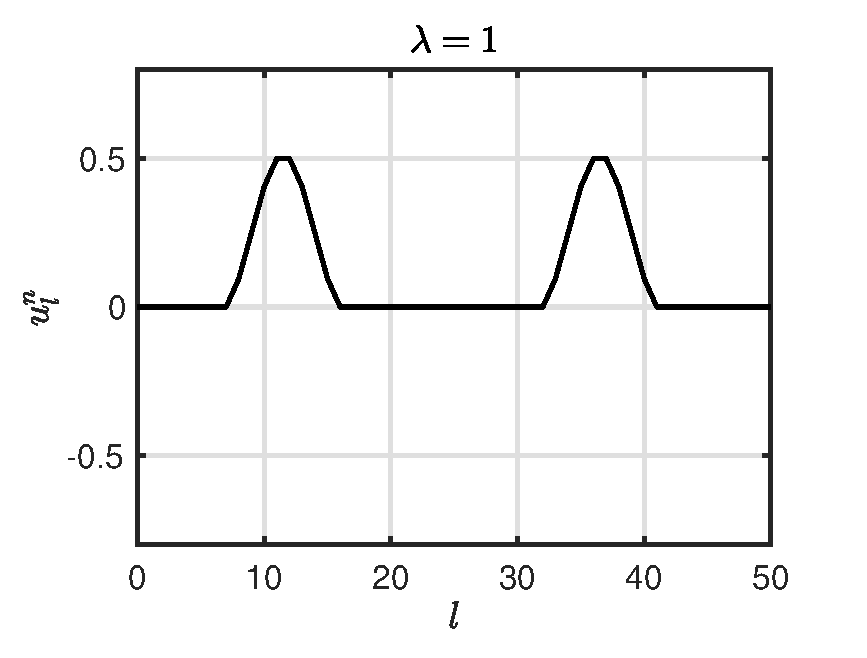
\includegraphics[width=0.3\textwidth]{ulnLambda1}}}
    \subfloat[]{\label{fig:lambda0.9}{ 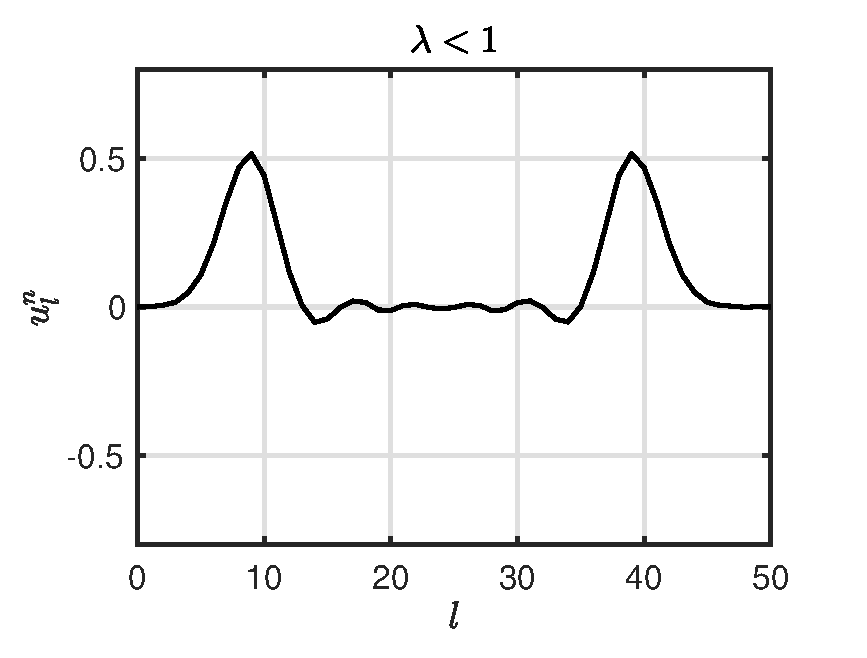
\includegraphics[width=0.3\textwidth]{ulnLambda09}}}
    \subfloat[]{\label{fig:lambda1.001}{ 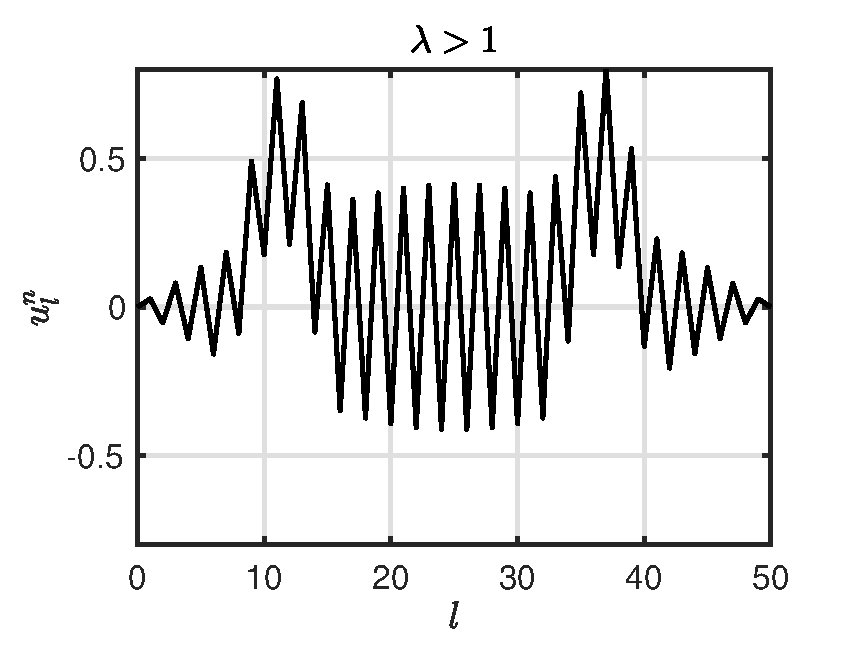
\includegraphics[width=0.3\textwidth]{ulnLambda1001}}}
    \caption{State $u_l^n$ with $N = 50$ and $f_\text{s} = 44100$ visualised $\sim\!100$ samples after excitation. (a) If $\lambda = 1$, the solution is exact. (b) If $\lambda < 1$ dispersive behaviour shows. (c) If $\lambda > 1$ the CFL condition in Eq. \eqref{eq:CFL} is not satisfied and the system is unstable.
    \label{fig:dispersion}}
\end{figure}

% discrete boundaries here?
Recalling \eqref{eq:lambdaDef} can rewrite Eq. \eqref{eq:CFL} in terms of grid spacing $h$ to get
\begin{equation}\label{eq:stabilityCond}
    h \geq ck.
\end{equation}
This shows that the CFL condition in \eqref{eq:CFL} puts a lower bound on the grid spacing, determined by the sample rate and wave speed. Usually, the following steps are taken to calculate $\lambda$
\begin{equation}\label{eq:orderOfCalcGrid}
    h := ck,\ \ N := \left\lfloor\frac{L}{h}\right\rfloor, \ \ h := \frac{L}{N}, \ \ \lambda := \frac{ck}{h}.
\end{equation}
In other words, condition \eqref{eq:stabilityCond} is first satisfied with equality and used to calculate integer $N$ according to Eq. \eqref{eq:numberOfIntervals}. Thereafter, $h$ is recalculated based on $N$ and used to calculate $\lambda$. The calculation of $\lambda$ in Eq. \eqref{eq:orderOfCalcGrid} can be compactly rewritten as
\begin{equation}\label{eq:compactLambda}
    \lambda = \frac{ck}{L}\cdot\left\lfloor\frac{L}{ck}\right\rfloor.
\end{equation}
The flooring operation causes the CFL condition in \eqref{eq:CFL} to not always be satisfied with equality and results in a reduced simulation quality described in the following section.

\subsection{Simulation Quality}\label{sec:quality}
As mentioned above, the Courant number $\lambda$ decides the quality of the simulation. Choosing $\lambda < 1$ will decrease this quality in two ways. Firstly, it will decrease the maximum frequency that the simulation is able to produce, i.e., it will decrease the bandwidth of the output sound of the system. See Figure \ref{fig:bandWidths}.

\begin{figure}[h]
    \centering
    \subfloat[]{\label{fig:bandwidth1}{ 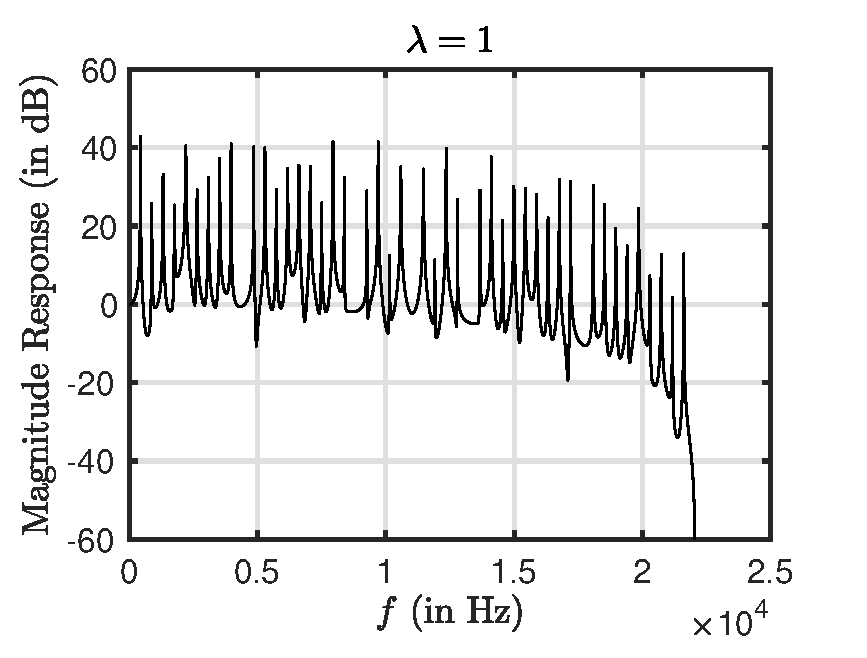
\includegraphics[width=0.3\textwidth]{bandwidthLambda1}}}
    \subfloat[]{\label{fig:bandwidth09}{ 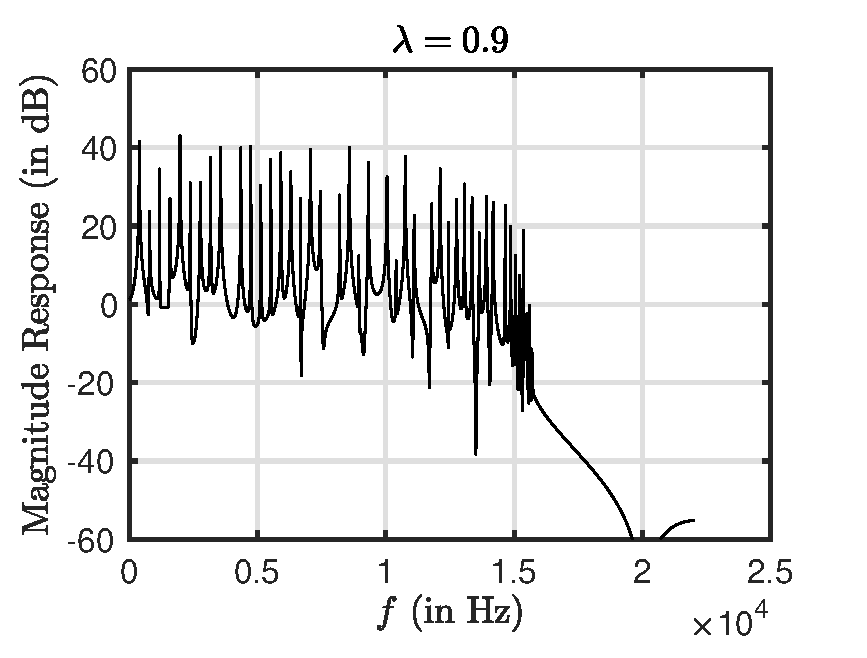
\includegraphics[width=0.3\textwidth]{bandwidthLambda09}}}
    \subfloat[]{\label{fig:bandwidth05}{ 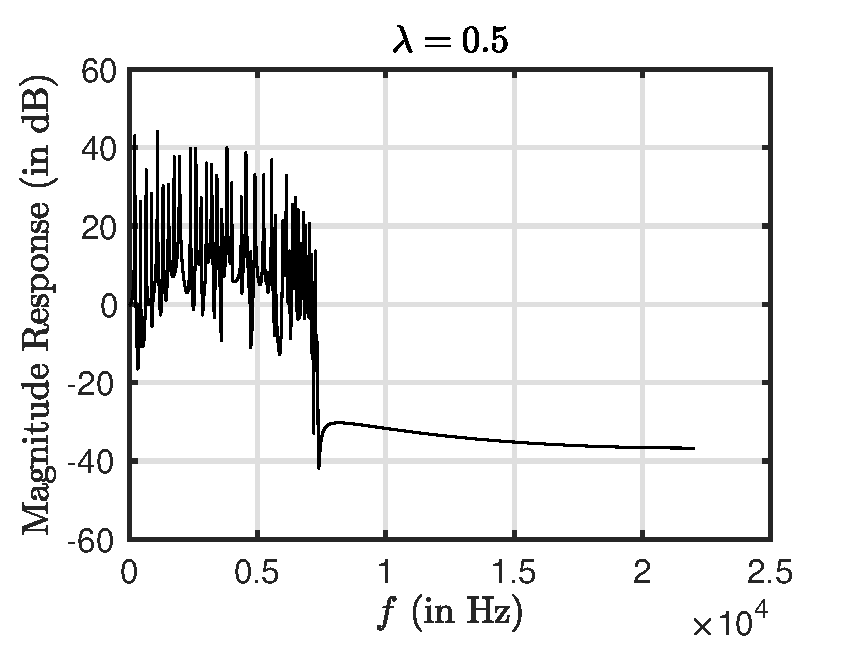
\includegraphics[width=0.3\textwidth]{bandwidthLambda05}}}
    \caption{Bandwidths of the simulation output %at $l = 16$ 
    with $f_\text{s} = 44100$ Hz and 
    %$N = 50$ excited with a raised cosine with a width of 5 at center-location $N = 25$. The Courant number is set to 
    (a) $\lambda = 1$, (b) $\lambda = 0.9$ and (c) $\lambda = 0.5$. 
    \label{fig:bandWidths}}
\end{figure}
%
By analysing the scheme in Eq. \eqref{eq:updateEq}, it can be shown that the maximum frequency produced by the system can be calculated using \cite[Chap. 6]{bilbao2009}
\begin{equation}\label{eq:fmax}
    f_\text{max} = \frac{f_\text{s}}{\pi} \sin^{-1}(\lambda).
\end{equation}
% shown in Figure \ref{fig:bandWidthFormula}.
%
Note that only a small deviation of $\lambda$ from condition \eqref{eq:CFL} already has a profound effect on the bandwidth of the output.
%
% \begin{figure}
% %% \reprintcolumnwidth is the same in preprint and reprint for
% %% ease of use for authors:
% \includegraphics[width=0.8\reprintcolumnwidth]{bandwidthPlot}
% \caption{\label{fig:bandWidthFormula}{The effect of the Courant number $\lambda$ on the output bandwidth. \SWcomment[This figure should probably be much more compact, if not removed altogether.]}}
% \end{figure} 
Secondly, choosing $\lambda < 1$ causes numerical dispersion. See Figures \ref{fig:lambda0.9} and \ref{fig:bandWidths}. Harmonic partials get closer together at higher frequencies (i.e. get more inharmonic) as $\lambda$ decreases, which is generally undesirable.

Apart from the recalculation of $\lambda$ due to the flooring operation in Eq. \eqref{eq:orderOfCalcGrid}, a reason that one would choose $\lambda < 1$ could be to decrease the total number of grid points used in the simulation by increasing $h$. This makes the simulation less computationally expensive, while keeping a desired wave speed $c$ and time step $k$. For 1-dimensional systems such as the 1D wave equation, this is rarely necessary.

\parskip 18pt
\section{Dynamic Parameters}\label{sec:dynamicParams}
This section describes how parameters could be made dynamic using FDTD methods and what this means for the simulation quality detailed in Section \ref{sec:quality}. %To clarify, for a parameter to be dynamic refers to its ability to vary over time while the simulation is running.  
To clarify, a \textit{dynamic} parameter refers to one that is time-varying while the simulation is running. 

% For the 1D wave equation used in Section \ref{sec:FDTD}, a property that could be interesting to make time-varying is the fundamental frequency $f_0$. If Dirichlet-type boundary conditions are used, as defined in Eqs. \eqref{eq:contDirichlet} and \eqref{eq:discreteDirichlet}, $f_0$ can be calculated according to
% \begin{equation}\label{eq:fundamentalFreq}
%     f_0 = \frac{c}{2L}\,.
% \end{equation}
% If $\lambda = 1$ in \eqref{eq:CFL} and thus condition \eqref{eq:stabilityCond} is satisfied with equality, $L/h$ in Eq. \eqref{eq:numberOfIntervals} is an integer and the flooring operation can be ignored. Substituting \eqref{eq:numberOfIntervals} into \eqref{eq:fundamentalFreq} yields
% \begin{equation}
%     f_0 = \frac{1}{2Nk}\ ,
% \end{equation}
% which shows that if $\lambda = 1$, $N$ solely decides the fundamental frequency of the simulation.

Usually when simulating musical instruments, the parameters of individual FDSs are fixed for the entire simulation. For the 1D wave equation used in Section \ref{sec:continuous}, these are the wave speed $c$ and time step $k$ (calculated from the sample rate $f_\text{s}$) from which the grid spacing $h$ and Courant number $\lambda$ are calculated. On top of this, the length $L$ can be changed, but as elaborated on in Section \ref{sec:dynamicParamsCont}, this can be directly translated to a change in $c$ through the fundamental frequency $f_0$. As $f_\text{s}$ is rarely changed \SWcomment[due to all sorts of issues], the sole parameter that could be interesting to make time-varying is $c$. 
% Modal synthesis is based on the addition of many sinusoids and is thus defined over the entire space. One can simply change the frequency of these sinusoids and 

% \begin{equation}\label{eq:modalSum}
%     u(x,t) = \sum_{m=1}^M C_m\sin(\omega_mt+\phi_m)\sin\Big(\frac{m\pi x}{L}\Big),
% \end{equation}
%
% The amount of modes that can be included also depends on a stability condition, but it is much easier to work with. One simply excludes modes that do not satisfy this condition. 
%
% Using FDTD methods, one uses a discrete set number of points making it hard to transition from one setting to the next.
As $c$ changes, several things need to be taken into account in a discrete setting. First of all, a change in $c$ causes a change in $\lambda$ according to Eq. \eqref{eq:compactLambda} affecting the simulation quality and bandwidth. Secondly, and more importantly, a change in $c$ could result in a change in $N$ through Eq. \eqref{eq:numberOfIntervals}. As $N$ directly relates to the number of grid points, this raises questions as to \textit{where} and especially \textit{how} one would add and remove points to the grid according to the now-dynamic wave speed.

A solution to the latter is to set and fix $N$ at the beginning of the simulation and tune $c$ away from the stability condition by decreasing it, such as done in \citep{Willemsen2019}. This would avoid problems with stability, as decreasing $c$ would continue to satisfy condition \eqref{eq:CFL}, but the simulation would end up with lower quality, exhibiting dispersive and bandlimiting effects as discussed in Section \ref{sec:quality}. In essence, decreasing the value of $c$ immediately translates to decreasing the value of $\lambda$ as $h$ and $k$ are left unchanged. On top of this, $c$ is limited by Eq. \eqref{eq:CFL} and increasing it beyond a certain value would render the system unstable.

The only way to circumvent the aforementioned undesirable effects such as dispersion and bandlimiting, is to somehow allow $N$ to be fractional or non-integer. This will remove the necessity of the flooring operation in Eq. \eqref{eq:numberOfIntervals} and Eq. \eqref{eq:compactLambda}, and will consequently satisfy the CFL condition in \eqref{eq:CFL} with equality at all times. Eq. \eqref{eq:fundamentalFreqCont} can then be rewritten in terms of $N$ by substituting Eq. \eqref{eq:numberOfIntervals} into Eq. \eqref{eq:fundamentalFreqCont} (using Eq. \eqref{eq:stabilityCond} satisfied with equality) yielding
\begin{equation}\label{eq:fundamentalFreq}
    f_0 = \frac{1}{2Nk}\ .
\end{equation}
This shows that if $\lambda = 1$, $N$, which is now not necessarily an integer, solely decides the fundamental frequency of the simulation. 

Even if a fractional $N$ would be possible, this still leaves the question of where and how to add and remove points to and from the grid. Furthermore, this change in grid size needs to happen in a smooth fashion so as not to create audible artefacts. 
%. To implement a physical model with dynamic parameters and an optimal simulation quality at all times,
This paper proposes a method that allows for a fractional $N$ and smoothly changes grid configurations \SWcomment[$\leftarrow$ elaborate on the fact that this means ``number of grid points"?] which the following section will describe. %The following section describes the requirements for such a method to successfully do this.

% Section \ref{sec:quality} shows several arguments for why these parameters should be fixed. The stability of the simulation relies on the parameters of the scheme and needs to be satisfied as close to the condition  When the stability condition is calculated,

% In this case we could initialise the system to have a wave speed of $c = 300$ m/s and a sample rate of $f_\text{s} = 44100$ Hz yielding $N = 147$ and $lambda = 1$ (satisfying condition \eqref{eq:CFL} with equality.

% Essentially $c$ is made time-varying / dynamic / changed on the fly $c^n$
% \subsection{Connection between $c$ and $L$ \SWcomment[(might be better as an appendix)]}\label{sec:f0}
% If Dirichlet-type boundary conditions are used, as defined in Eqs. \eqref{eq:contDirichlet} and \eqref{eq:discreteDirichlet}, the fundamental frequency $f_0$ of the 1D wave equation can be calculated according to
% \begin{equation}
%     f_0 = \frac{c}{2L}\,,
% \end{equation}
% from which one can see that, in terms of fundamental frequency a halving the length is identical to doubling the wave speed. 
% If $\lambda = 1$ in \eqref{eq:CFL} and thus condition \eqref{eq:stabilityCond} is satisfied with equality, $L/h$ in Eq. \eqref{eq:numberOfIntervals} is an integer and the flooring operation can be ignored. Substituting \eqref{eq:numberOfIntervals} into \eqref{eq:fundamentalFreq} yields
% \begin{equation}
%     f_0 = \frac{1}{2Nk}\ ,
% \end{equation}
% which shows that if $\lambda = 1$, $N$ solely decides the fundamental frequency of the simulation.
\parskip 18pt
\section{The Dynamic Grid}
By now, it is hopefully clear to the reader why dynamic parameters would make an interesting case in the field of physical modelling, and why dynamic grids would be a good solution to undesirable behaviour such as a decrease in bandwidth and increase in numerical dispersion discussed in Section \ref{sec:quality}. %This section will describe the problems that arise when adding and removing grid points. Afterwards, some iterations done over the course of this project and their drawbacks will be shown, leading up to the final implementation of the dynamic grid. 

% The first questions that need to be answered are ``where to add points?" and ``how to add points?" The problems when doing this range from artifacts or auditory `clicks' in the output sound to ``exploding" systems due to artificial injection of energy. 
First, this section will list the requirements of a method that dynamically changes FDTD grid configurations. Then, the iterations done over the course of this project will briefly be described, the details of each can be found in Appendix \ref{app:A}. \SWcomment[(I think I might remove the iterations and appendix actually..)] Finally, the proposed method will be described in detail and summarised in the end.

\subsection{Method requirements}\label{sec:methodReq}
Ideally, a method that dynamically changes the grid size of finite-difference schemes should
\begin{enumerate}
    \item generate an output with a fundamental frequency $f_0$ %described by Eq. \eqref{eq:fundamentalFreq} 
    which is linearly proportional to $c$ ($f_0 \propto c$),
    \item allow for a fractional $N$ to smoothly transition 
    %between different $f_0$s,
    %\item smoothly transition 
    between different grid configurations so that no auditory artefacts are present in the output sound,
    \item generate an output containing harmonic partials -- or modes -- which are integer multiples of the fundamental ($f_p = f_0 p$ with integer $p$),
    \item generate an output with $\lfloor N\rfloor-1$ modes corresponding to the number of moving points of the system ($p = [1, \hdots, \lfloor N\rfloor-1]$),\\
    \item work in real time.
\end{enumerate}
The last requirement is an optional one, but in order for the final implementation to be ``playable'', this is necessary. 
%
% The total amount of modes is expected to be equal to $N-1$ corresponding to the total number of moving grid points (points excluding the boundary).
%As the variables $c$, $h$, $\lambda$ and $N$ are now time-varying, a superscript $n$ or $n-1$ is added when necessary. If omitted, a time index $n$ is assumed.

\subsection{Iterations \SWcomment[(optional section)]}\label{sec:iterations} 
One method that could be used to go from one grid configuration to the next is full-grid interpolation as described in \citep[Chap. 5]{bilbao2009}. However, this method essentially has a lowpassing effect on the entire system state and can cause `clicks' in the output sound due to the interpolation. A (much) higher sample rate could be used to avoid these issues, but this would render this method impossible to work in real time.

Another method is to add and remove points at the boundary using an interpolated boundary condition, the possibility of which has been briefly mentioned in \citep[p. 145]{bilbao2009}. If the boundary is fixed through Eq. \eqref{eq:contDirichlet}, the state at this location will always be $0$ and potentially allows for smooth entry and exit of grid points at this location. This method can be seen analogous to tuning a guitar string where string-material enters and leaves the playable part of the string at the nut, the boundary. The interpolated nature of the boundary does allow for a ``fractional" $N$ as described in Section \ref{sec:dynamicParams} and has a fundamental frequency calculated using \eqref{eq:fundamentalFreq}. %removing the flooring operation in Eq. \eqref{eq:compactLambda} and always satisfying the CFL condition with equality. \SWcomment[This has the added feature that $L/h$ in Eq. \eqref{eq:numberOfIntervals} is an integer and the flooring operation can be ignored. Substituting Eq. \eqref{eq:numberOfIntervals} into Eq. \eqref{eq:fundamentalFreqCont} (using Eq. \eqref{eq:stabilityCond} satisfied with equality) yields
%\begin{equation}%\label{eq:fundamentalFreq}
%     f_0 = \frac{1}{2Nk}\ ,
% \end{equation}
% which shows that if $\lambda = 1$, $N$, which is now not necessarily an integer, solely decides the fundamental frequency of the simulation.] 
Although informal testing shows that adding points to the grid can happen smoothly, removing points smoothly is more challenging. This is due to the fact that the grid point at the boundary will be moving right before it is removed and its displacement needs to (somehow) smoothly be reduced to 0 to satisfy the fixed boundary condition in Eq. \eqref{eq:contDirichlet}. %\SWcomment[$\leftarrow$ if simply supported condition is mentioned here] Even though the $\delta_{xx}u$ part of this condition can be easily satisfied, the $u=0$ part can not.

\subsection{Proposed Method}\label{sec:proposedMethod}
This section introduces the proposed method of dynamically and smoothly changing the grid to account for dynamic parameter changes. To avoid the issues of adding and removing points at the boundary due to boundary conditions, they can be added or removed along the grid instead. For the sake of simplicity, the location is chosen to be the center of the system. %\SWcomment[At the end of this section, the location exhibiting the best behaviour will be shown.] 
In the following, the location of a grid point (in m from the left boundary) $i$ (such as $i = u_0$) at time index $n$ is denoted by $x_i^n$. 

\subsubsection{System Setup}\label{sec:systSetup}
Consider a grid function, $u_l^n$ with integer $M_u = \lceil 0.5L/ck\rceil $ (or simply $M$ below for brevity) \SWcomment[($\lceil \cdot \rceil$ denoting the ceiling operation)] and $w_l^n$ with integer $M_w = \lfloor 0.5L/ck\rfloor$, i.e., half the number of points allowed by the stability condition, plus one for overlap (see Figure \ref{fig:twoFreeStrings}). The following boundary conditions are then imposed:
\begin{subequations}\label{eq:halfStringBoundaryCond}
    \begin{align}
        u_0^n = w_{M_w}^n &= 0,\quad \text{(Dirichlet)}\label{eq:halfStringBoundaryCondDirichlet}\\
        \delta_{x\cdot}u_M^n = \delta_{x\cdot}w_0^n &= 0.\, \quad\text{(Neumann)}, \label{eq:halfStringBoundaryCondNeumann}
    \end{align}
\end{subequations}
i.e., the outer boundaries are fixed and the inner boundaries are free.
% \begin{figure}[h]
% \centerline{\includegraphics[width=\columnwidth]{twoFreeStrings.eps} }
% \caption{\label{fig:twoFreeStrings}{Two (1D wave) systems connected at one of their boundaries.}}
% \end{figure}
%
% \baselineskip=12pt

\begin{figure}[hp]
    \centering
    \subfloat[]{\label{fig:twoFreeStrings}{ 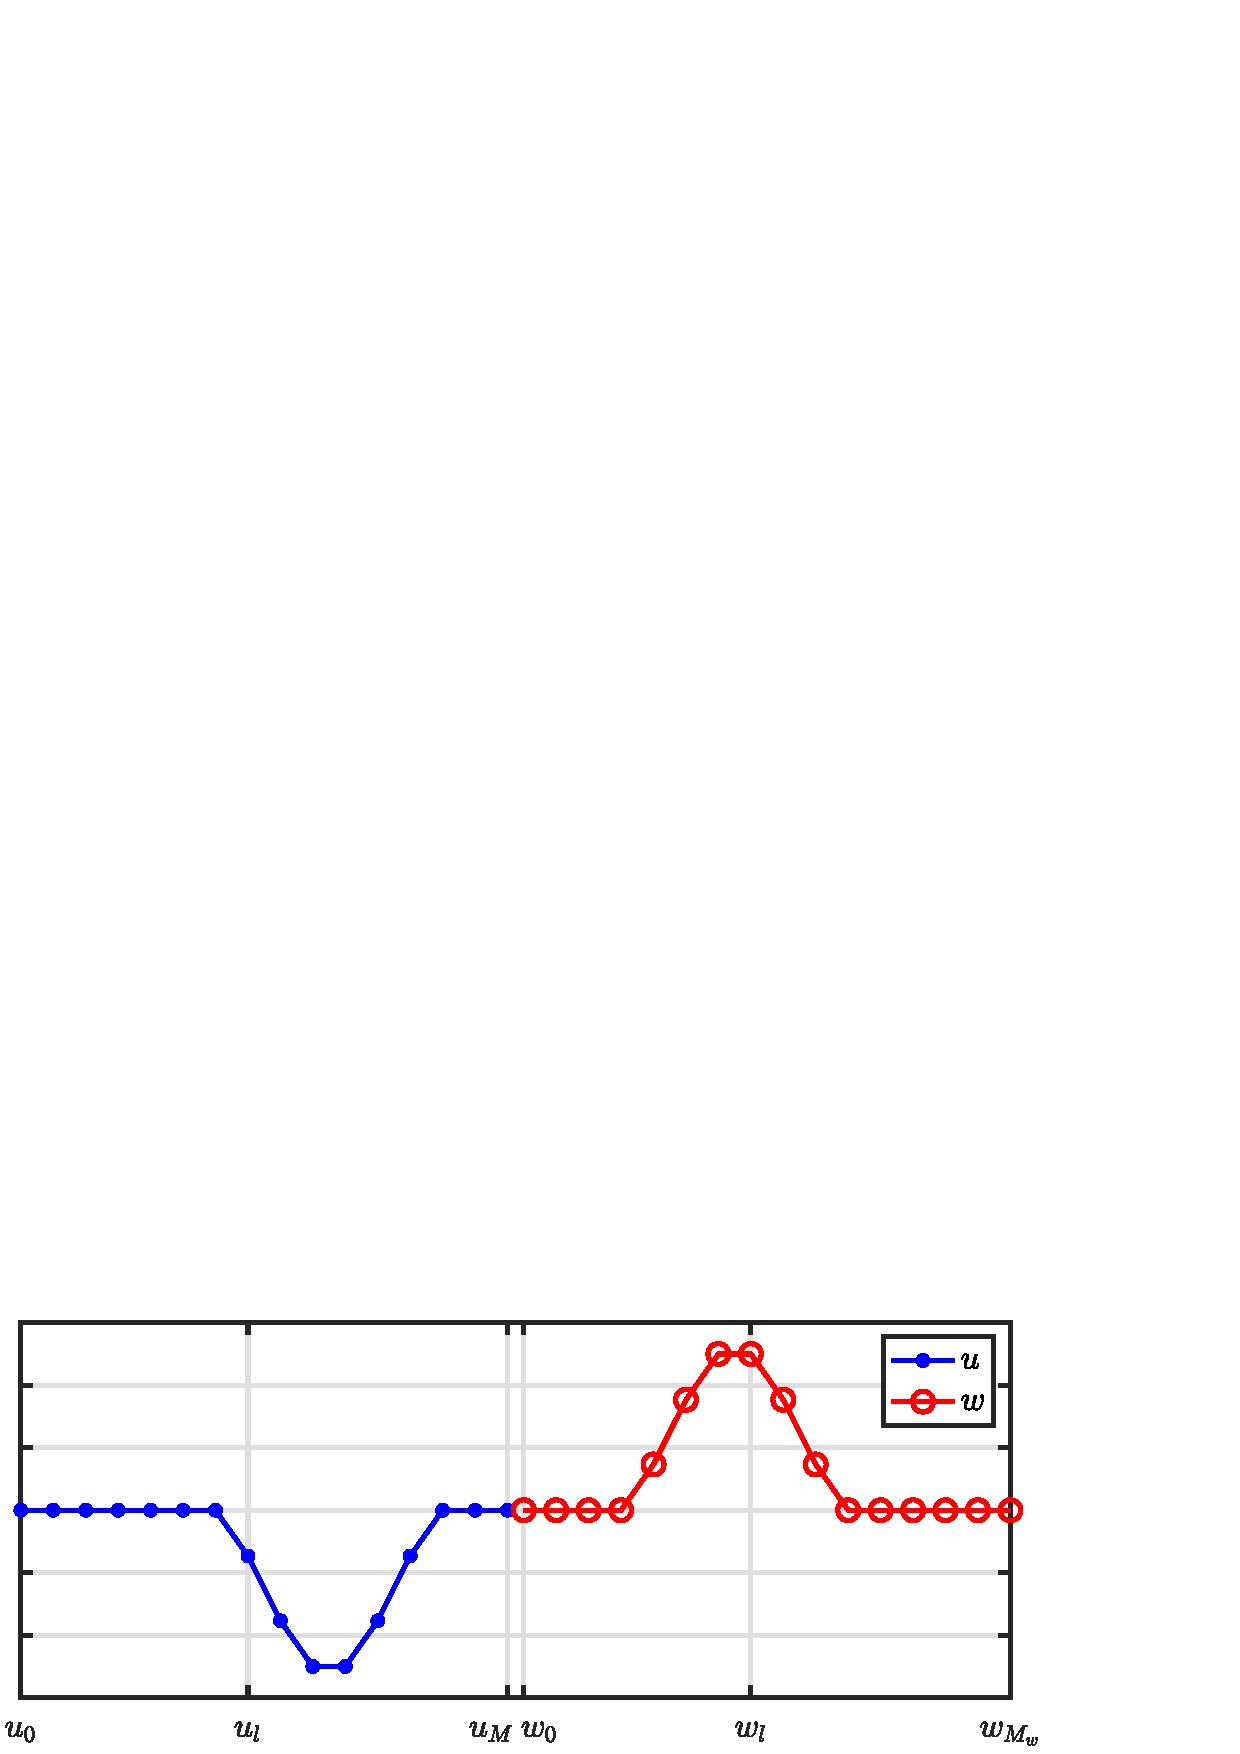
\includegraphics[width=0.8\columnwidth]{twoFreeStringGridMove}}}\\
    \subfloat[]{\label{fig:twoFreeStringsGridMoveZoomed}{ 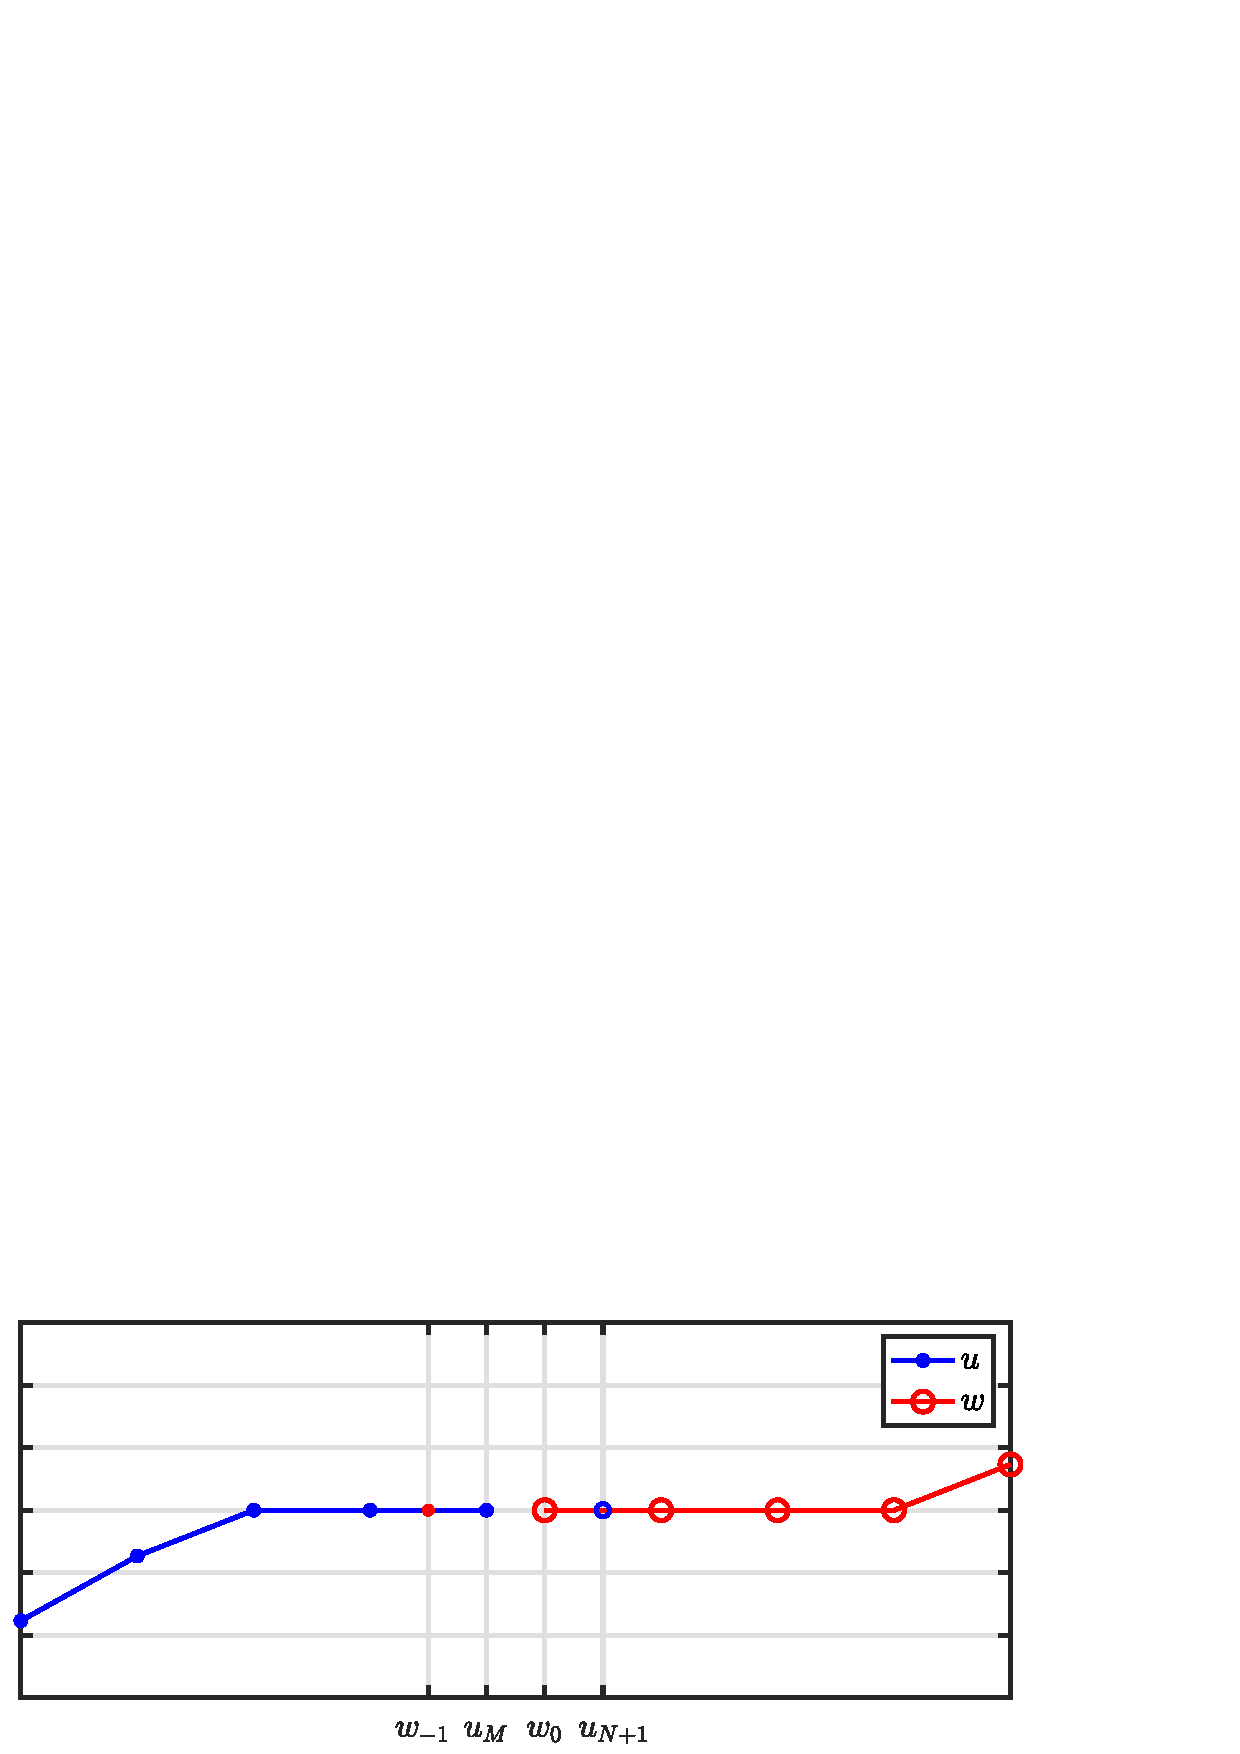
\includegraphics[width=0.8\columnwidth]{twoFreeStringGridMoveZoomed}}}\\
    \subfloat[]{\label{fig:twoFreeStringsGridZoomed2}{ 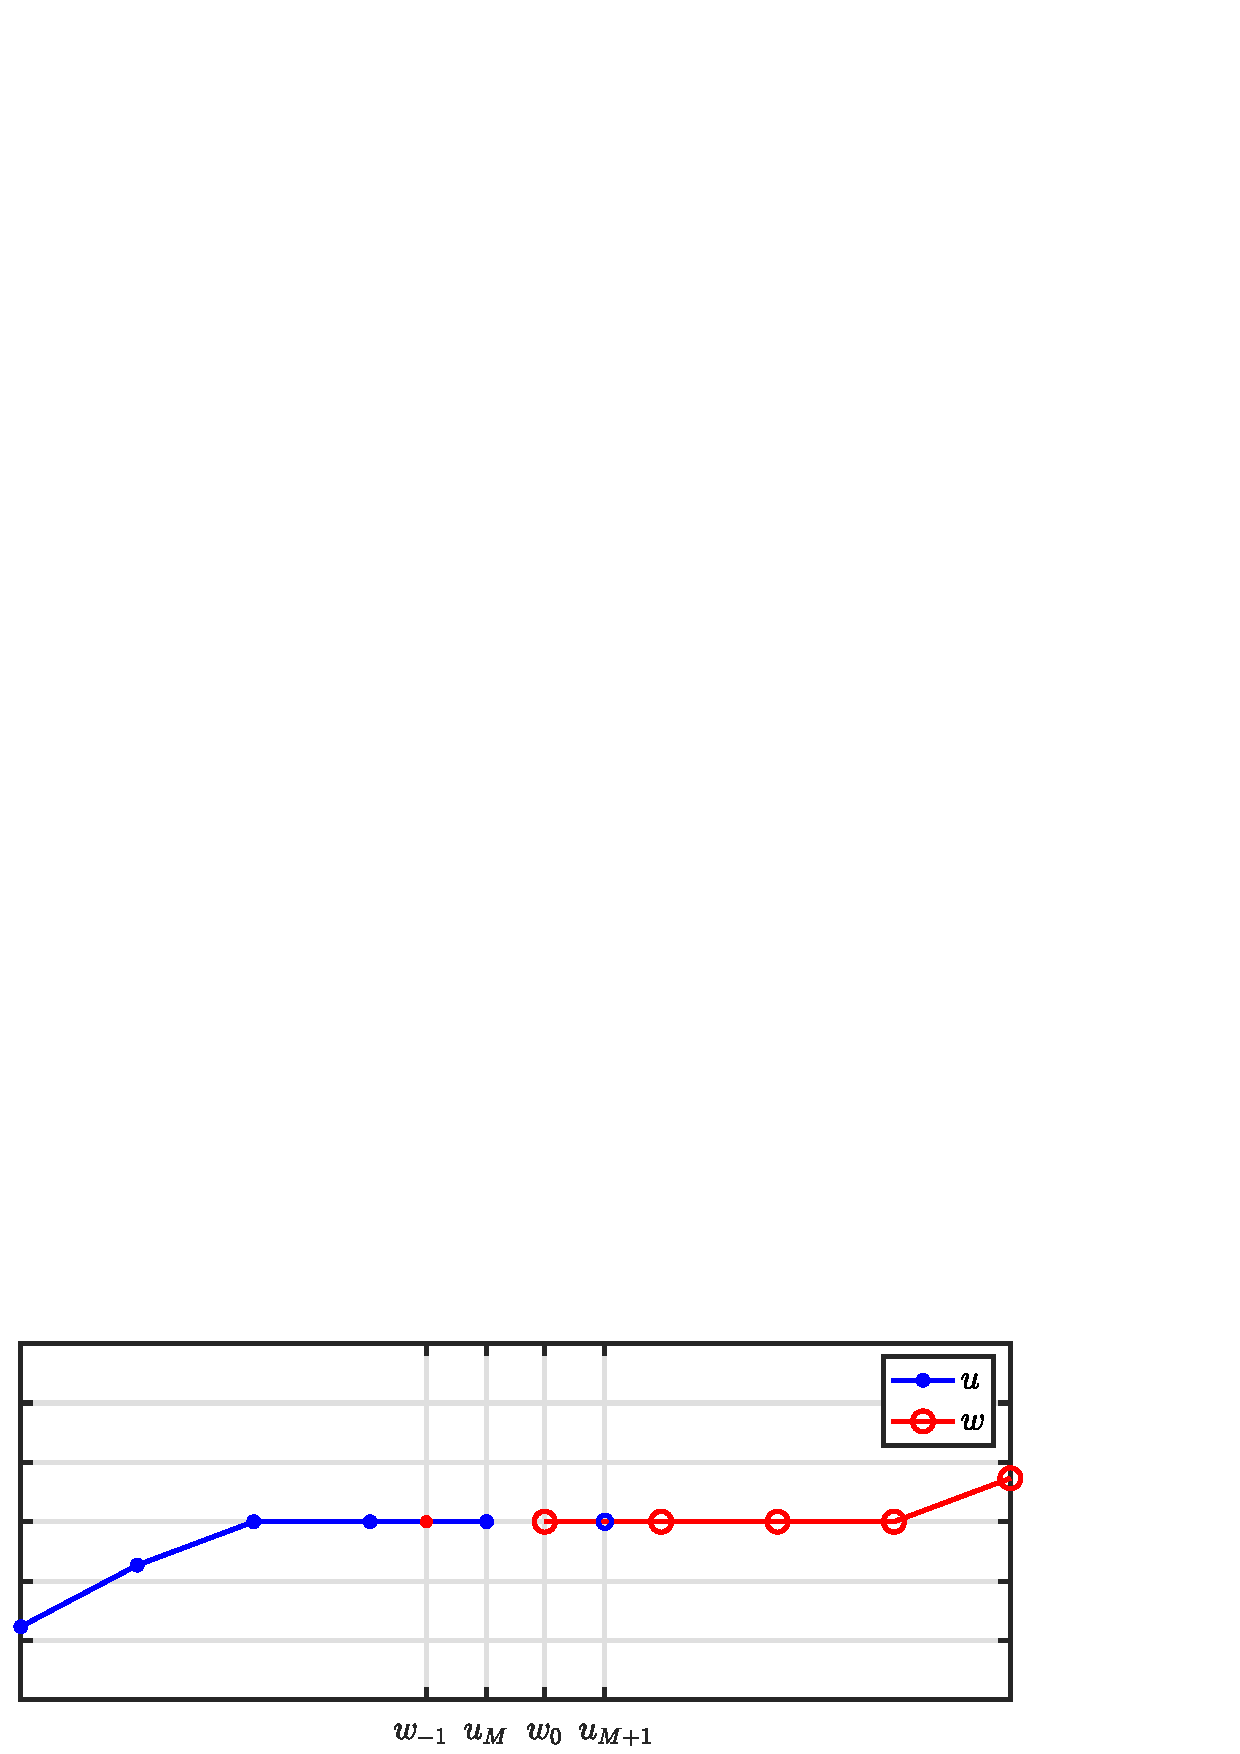
\includegraphics[width=0.8\columnwidth]{twoFreeStringGridMoveZoomed2}}}
    \caption{Illustration of the proposed method. In all figures, the x-axis shows the location (in m) of the respective grid points (fx. $x_{u_l^n}$), but the $x$ and $n$ are omitted for brevity. (a) Locations of the states of two (1D wave) systems connected at the inner boundary ($N = 30$, $x_{u_M}^n = x_{w_0}^n$). (b) When $c$ -- and consequently $h$ -- are decreased and the positions of the grid points change ($N = 30.5$, $x_{u_M}^n \neq x_{w_0}^n$). (c) Figure \ref{fig:twoFreeStrings} zoomed-in around $x_{u_M}^n$ and $x_{w_0}^n$. The states at the inner boundaries $u_M^n$ and $w_0^n$ are shown together with virtual grid points $u_{M+1}^n$ and $w_{-1}^n$.}
\end{figure}
%
The systems can then be connected at the inner boundaries ($u_M^n$ and $w_0^n$) using a rigid connection, i.e. \SWcomment[(only valid if $x_{u_M}^n = x_{w_0}^n$)],
\begin{equation}\label{eq:rigid}
    u_M^n = w_0^n,\quad \forall n.
\end{equation}
Essentially, the complete system is divided into two separate systems connected at the inner boundary. 

With these boundary conditions imposed, the following, state vectors can be defined:
\begin{equation}
    \begin{aligned}\label{eq:separateStateVectors}
     \mathbf{u}^n &= [u_1^n, \hdots, u_M^n]^T, \\
     \mathbf{w}^n &= [w_0^n, \hdots, w_{M_w-1}^n]^T,
    \end{aligned}
\end{equation}
with $T$ denoting the transpose operation, and have $M$ and $M_{w}$ points respectively. Note that the outer boundaries are excluded as they are 0 at all times. The vector concatenating \eqref{eq:separateStateVectors} is then defined as 
\begin{equation}\label{eq:fullState}
    \U^n = \begin{bmatrix}
        \mathbf{u}^n \\
        \mathbf{w}^n
    \end{bmatrix}.
\end{equation}
Note that the vectors in \eqref{eq:separateStateVectors} and \eqref{eq:fullState} also exist at the next ($n+1$) and previous ($n-1$) time indices. The system of FDSs will now be
\begin{equation}
    \begin{cases}\label{eq:systemHalfStrings}
        \delta_{tt}u_l^n = c^2\delta_{xx}u_l^n + J(x_{u_M}^n)F\\
        \delta_{tt}w_l^n = c^2\delta_{xx}w_l^n - J(x_{w_0}^n)F
    \end{cases}
\end{equation}
with spreading operator
\begin{equation}
    J(x_i) =
    \begin{cases}
        \frac{1}{h}, & l = l_i = \lfloor x_i/h\rfloor\\
        0,& \text{otherwise}
    \end{cases}
\end{equation}
and the effect of the connection \SWcomment[(``connection force", but not really as it isn't in N)] $F$ (in m$^2$/s$^2$).
%
Expanding the spatial operators in system \eqref{eq:systemHalfStrings} at inner boundaries $u_M^n$ and $w_0^n$, recalling the Neumann condition in  \eqref{eq:halfStringBoundaryCondNeumann} and the definition for the virtual grid points needed for this condition in Eq. \eqref{eq:neumannSolution} yields
\begin{equation}\label{eq:expandedSystem}
    \begin{cases}
        \delta_{tt}u_M^n = \frac{c^2}{h^2}(2u_{M-1}^n-2u_M^n) + \frac{1}{h}F\\
        \delta_{tt}w_0^n = \frac{c^2}{h^2}(2w_1^n-2w_0^n) - \frac{1}{h}F.
    \end{cases}
\end{equation}
Because of Eq. \eqref{eq:rigid}, it is also true that $\delta_{tt}u_M^n = \delta_{tt}w_0^n$, and $F$ can be calculated by setting the right side of the equations in \eqref{eq:systemHalfStrings} equal to each other:
\begin{align*}
     \frac{c^2}{h^2}(2u_{M-1}^n-2u_M^n) + \frac{1}{h} F&= 
     \frac{c^2}{h^2}(2w_1^n-2w_0^n) - \frac{1}{h} F\nonumber\\
    % \frac{2}{h}F &= \frac{c^2}{h^2}(2w_1^n - 2u_{M-1}^n)\nonumber\\
    F &= h \frac{c^2}{h^2}(w_1^n - u_{M-1}^n)
\end{align*}
Substituting this into system \eqref{eq:expandedSystem} after expansion of the second-time derivative yields the update of the inner boundaries
% \begin{equation}
\begin{subnumcases}{\!\!\!\!\!\!\!\!\!\!\!\!\!\!\label{eq:resultOneConnectedPoint}}
    u^{n+1}_M = 2u_M^n - u_M^{n-1} + \lambda^2(u_{M-1}^n-2u_M^n+w_1^n)\label{eq:resultUM}\\
    w^{n+1}_0 = 2w_0^n - w_0^{n-1} + \lambda^2(u_{M-1}^n-2w_0^n+w_1^n)\label{eq:resultw0}
\end{subnumcases}
% \end{equation}
which, (again, recalling Eq. \eqref{eq:rigid}) are indeed equivalent expressions for the connected point. Here, $w_1^n$ in Eq. \eqref{eq:resultUM} acts as virtual grid point $u_{M+1}^n$ and $u_{M-1}^n$ in \eqref{eq:resultw0} as virtual grid point $w_{-1}^n$, essentially connecting the two systems using the state of one in the update of the other.

\subsubsection{Changing the Grid}
The previous section describes the case in which the stability condition is satisfied with equality, i.e, when $1/ck$ is an integer and $x_{u_M}^n = x_{w_0}^n$. The locations of the outer boundaries $x_{u_0}^n$ and $x_{w_{M_w}}^n$ are fixed, i.e.
\begin{equation*}
    x_{u_0}^n = x_{u_0}^0 \quad \text{and}\quad x_{w_{M_w}}^n = x_{w_{M_w}}^0 \quad \forall n.
\end{equation*}
If the wave speed $c$ is then decreased, and consequently the grid spacing $h$ according to $h=ck$, all other points move towards their respective outer boundary (see Figure \ref{fig:twoFreeStringsGridMove}). Calculating $h$ this way allows this method to always satisfy the CFL condition in Eq. \eqref{eq:CFL} with equality, as is the case with the previous iteration described in \ref{sec:iterations}.

% \begin{figure}[h]
% \centerline{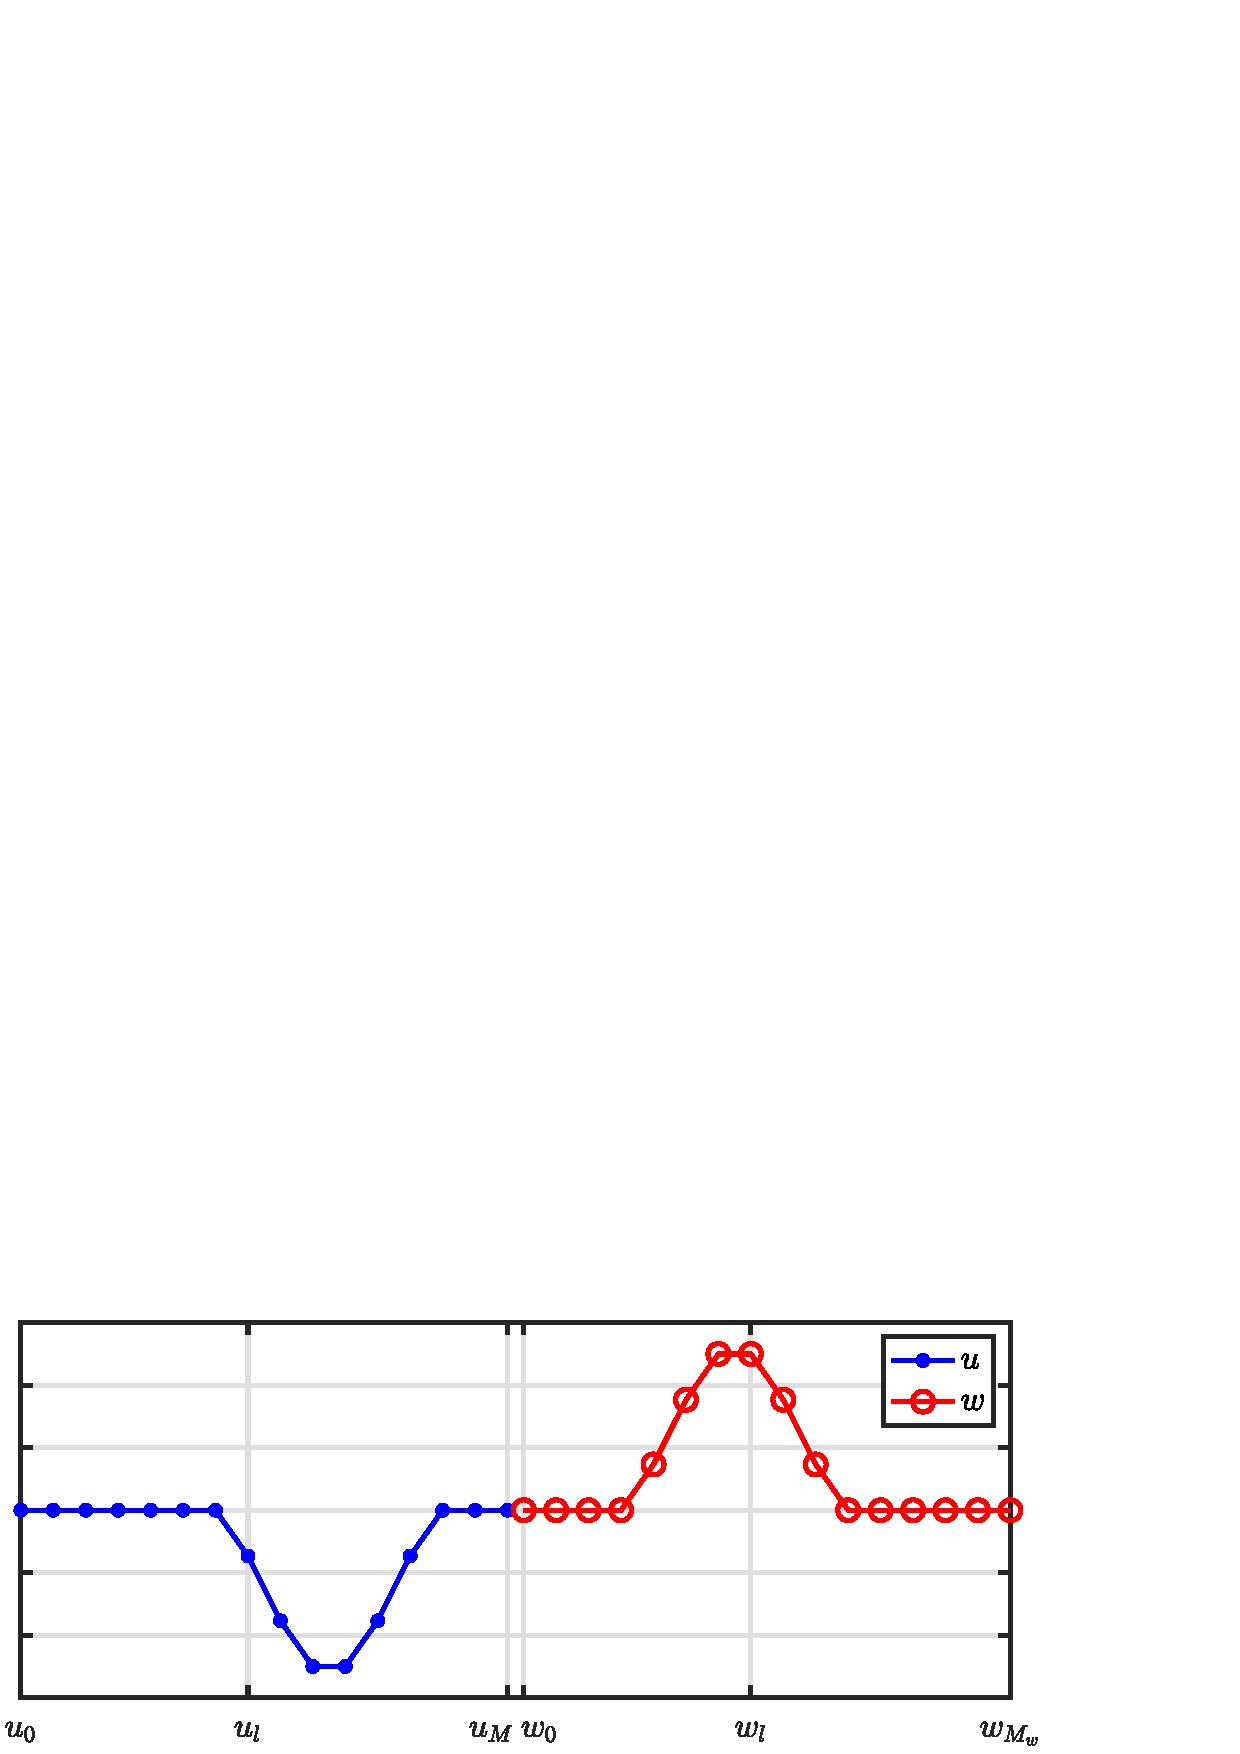
\includegraphics[width=\columnwidth]{twoFreeStringGridMove} }
% \caption{\label{fig:twoFreeStringsGridMove}{When the grid changes ($N = 30.5$). The x-axis shows the location (in m) of the respective grid points (fx. $x_{u_l^n}$), but the $x$ is omitted for clarity.}}
% \end{figure}
%
As mentioned above, the state of $\mathbf{w}^n$ (from \eqref{eq:separateStateVectors}) can be used to calculate the virtual grid point needed at the right boundary of $\mathbf{u}^n$ and vice versa. If the inner boundaries are not overlapping (i.e., $x^n_{u_M} \neq x^n_{w_0}$) a Lagrangian interpolator $I(x_i)$ at location $x_i$ from the left boundary (in m) can be used to calculate the value of this virtual grid point. The interpolator $I$ is a row-vector the size of $\mathbfcal{U}^n$ (from Eq. \eqref{eq:fullState}) its values depending on what interpolation order is used. In the following, the distance between the inner boundaries is defined as
\begin{equation}\label{eq:alphaDef}
    \alpha = \alpha^n = \frac{x^n_{w_0} - x^n_{u_M}}{h}\,,
\end{equation}
and for clarity, $I$ and $\mathbfcal{U}^n$ are indexed by $m$.
Applying the interpolator to $\mathbfcal{U}^n$ yields
\begin{subequations}\label{eq:interpolationGeneral}
    \begin{align}
        u_{M+1}^n &= I^\flip(x^n_{u_{M+1}})\mathbfcal{U}^n% = (1-\alpha)w_1^n + \alpha w_0^n
        \\
        w_{-1}^n &= I(x^n_{w_{-1}})\mathbfcal{U}^n,% = (1-\alpha)u_{M-1}^n + \alpha u_M^n
    \end{align}
\end{subequations}
where $I^\flip$ is a flipped and shifted version of $I$. \SWcomment[$\leftarrow$ further explanation needed here..]
% where
% \begin{equation}
%     \alpha = \frac{x_{w_0} - x_{u_M}}{h},
% \end{equation}
% and grid-point locations $x_{u_{M+1}}$ and $w_{-1}$. Note that when $h$ changes the connected points start to move away from each other.
%
If linear interpolation is used, 
\begin{subequations}\label{eq:linearInterp}
\begin{equation}
    I_1(x_i) = 
    \begin{cases}
        (1-\alpha) & m = m_i \\\alpha & m = m_i + 1\\
        0 & \text{otherwise}
    \end{cases}
\end{equation}
and
\begin{equation}
    I_1^\flip(x_i) = 
    \begin{cases}
        \alpha & m = m_i^\flip \\(1-\alpha) & m = m_i^\flip + 1\\
        0 & \text{otherwise}
    \end{cases}
\end{equation}
\end{subequations}
with $m_i = \lfloor x_i/h\rfloor$ and $m_i^\flip = \lfloor x_i/ h+(1-\alpha) \rfloor$. The shift in the latter is necessary to transform the location to the right indices of $\mathbfcal{U}^n$. \SWcomment[$\leftarrow$ more explanation here] Substituting \eqref{eq:linearInterp} into \eqref{eq:interpolationGeneral} yields
\begin{subequations}
    \begin{align}
        u_{M+1}^n &= I_1^\flip(x^n_{u_{M+1}})\mathbfcal{U}^n = \alpha w_0^n
        + (1-\alpha)w_1^n,\\
        w_{-1}^n &= I_1(x^n_{w_{-1}})\mathbfcal{U}^n = (1-\alpha)u_{M-1}^n + \alpha u_M^n.
    \end{align}
\end{subequations}

Also see Figure \ref{fig:twoFreeStringsGridZoomed}.
% \begin{figure}[h]
% \centerline{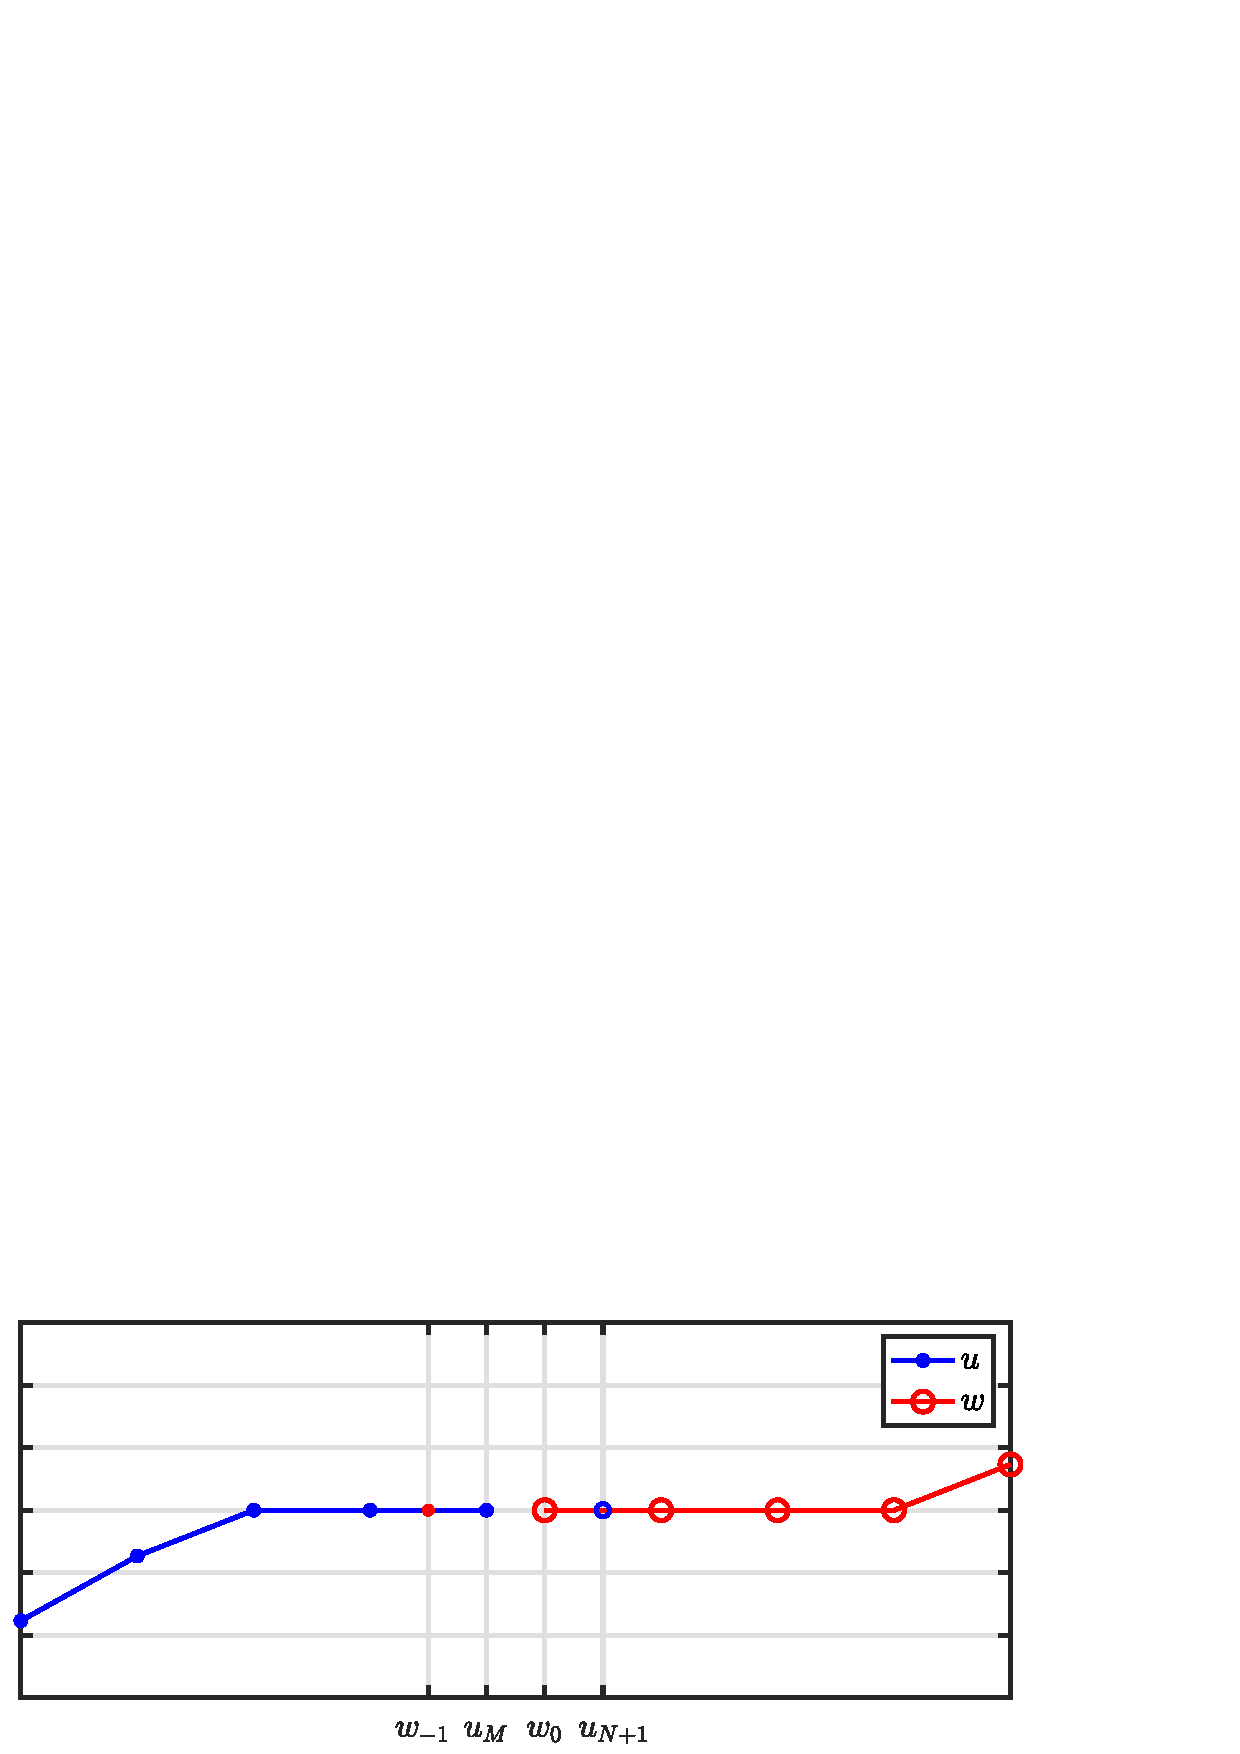
\includegraphics[width=\columnwidth]{twoFreeStringGridMoveZoomed} }
% \caption{\label{fig:twoFreeStringsGridZoomed}{When the grid changes (zoomed). The states at the inner boundaries $u_M$ and $w_0$ are shown together with virtual grid points $u_{M+1}$ and $w_{-1}$.}}
% \end{figure}
%
Using $I_1$, analysis of the output shows that the expected fundamental frequency $f_0$ is slightly higher when interpolation needs to happen than the one expected when using Eq. \eqref{eq:fundamentalFreq}. Furthermore, modes higher than $f_\text{s} / 4$ would follow an odd pattern up when decreasing the wavespeed, opposite of what is expected.

One could extend the range of interpolation by one point to each side, using a cubic Lagrange interpolator instead. Though this would require $w_{-1}^n$ to calculate $u_{M+1}^n$ and vice versa, it is possible to solve this by treating the interpolation equations as a system of linear equations. Analysis of this method, though yielding a correct $f_0$ at all times, shows similar behaviour to the linear interpolation, with odd behaviour regarding to modes higher than $f_\text{s}/4$.

Much better behaviour is observed when points of both $\mathbf{u}^n$ and $\mathbf{w}^n$ are used to calculate the values of the virtual grid points. This means to also use $u_M^n$ to calculate $u_{M+1}^n$ and $w_0^n$ for $w_{-1}^n$. Now, the locations of the grid points used in the interpolation are not equidistant and a custom Lagrangian interpolator needs to be created. The lowest order interpolator that can be used here is the quadratic interpolator $I_2$ and when applied to Eq. \eqref{eq:fullState} yields
\begin{subequations}\label{eq:connectionInterpol}
\begin{align}
    &\begin{aligned}\label{eq:calcUMP1}
        u_{M+1}^n &= I_2^\flip(x^n_{u_{M+1}})\mathbfcal{U}^n\\
        &= \frac{\alpha - 1}{\alpha + 1}u_{M}^n + w_0^n - \frac{\alpha - 1}{\alpha + 1}w_1^n
    \end{aligned}\\
    &\ \ \begin{aligned}\label{eq:calcWM1}
        w_{-1}^n &= I_2(x^n_{w_{-1}})\mathbfcal{U}^n \\
        &=-\frac{\alpha - 1}{\alpha + 1}u_{M-1}^n + u_{M}^n+ \frac{\alpha - 1}{\alpha + 1}w_{0}^n.
    \end{aligned}
\end{align}
\end{subequations}
% where
% \begin{equation}\small
% \begin{gathered}\label{eq:interpolationCoeffs}
%     \alpha_\text{I} = \frac{\alpha(\alpha - 1)(\alpha - 2)}{-6}, \quad \beta_\text{I} = \frac{(\alpha - 1)(\alpha + 1)(\alpha - 2)}{2},\\
%     \gamma_\text{I} = \frac{\alpha(\alpha + 1)(\alpha - 2)}{-2}, \quad \text{and} \quad\delta_\text{I} = \frac{\alpha(\alpha + 1)(\alpha - 1)}{6}\,.
% \end{gathered}
% \end{equation}
% Treating \eqref{eq:connectionInterpol} as a system of linear equations, the virtual grid points $u_{M+1}^n$ and $w_{-1}^n$ can be solved for using
% \begin{equation}\label{eq:linSystSolution}
%     \begin{bmatrix}
%     u_{M+1}^n \\
%     w_{-1}^n
%     \end{bmatrix}
%     =
%     \mathbfcal{A}\begin{bmatrix}
%     \alpha_\text{I} w_2^n+ \beta_\text{I}w_1^n + \gamma_\text{I}w_0^n \\
%     \alpha_\text{I} u_{M-2}^n + \beta_\text{I}u_{M-1}^n + \gamma_\text{I} u_{M}^n
%     \end{bmatrix},
% \end{equation}
% where
% \begin{equation}\label{eq:Amat}
%     \mathbfcal{A} = \begin{bmatrix}
%          1 & -\delta_\text{I} \\
%          -\delta_\text{I} & 1
%     \end{bmatrix}^{-1}.\nonumber
% \end{equation}
% where
% \begin{equation}\nonumber
%     \mathbfcal{A} = \begin{bmatrix}
%          1 & -\delta_\text{I} \\
%          -\delta_\text{I} & 1
%     \end{bmatrix},
% \end{equation}
% and
% \begin{equation}\nonumber
%     \mathbf{v} = \begin{bmatrix}
%     \alpha_\text{I} w_2^n+ \beta\text{I}w_1^n + \gamma\text{I}w_0^n \\
%     \alpha_\text{I} u_{M-2}^n + \beta\text{I}u_{M-1}^n + \gamma u_{M}^n
%     \end{bmatrix}.
% \end{equation}
As will be shown in Section \ref{sec:results}, quadratic interpolation yields the expected fundamental frequency at all times. One can show that when $N$ is an integer, and thus $\alpha = 0$, Eqs. \eqref{eq:calcUMP1} and \eqref{eq:calcWM1} can be substituted as $w_1^n$ and $u_{M-1}^n$ into Eqs. \eqref{eq:resultUM} and \eqref{eq:resultw0} respectively (as these acted as virtual grid points $u_{M+1}^n$ and $w_{-1}^n$). Then recalling Eq. \eqref{eq:rigid} it can be seen that the system is reduced to \eqref{eq:resultOneConnectedPoint}. % also when interpolation needs to happen.

\subsubsection{Adding and removing Grid Points}
When $c$, and consequently $h$, is decreased and the inner boundary points surpass the virtual points (i.e. $x_{u_M}^n \leq x_{w_{-1}}^n$ and $x_{w_0}^n \geq x_{u_{M+1}}^n$) and $\lfloor N^n\rfloor > \lfloor N^{n-1}\rfloor$, a point is added to the right boundary of $\mathbf{u}$ and the left boundary of $\mathbf{w}$ (for both time indices $n$ and $n-1$) in an alternating fashion: 
\begin{equation}\label{eq:addingPoint}
        \begin{cases}\mathbf{u}^n = [\mathbf{u}^n, I_3(x_{u_{M+1}}^n)\mathbf{v}^n]^T & \text{if $\lfloor N^n\rfloor $ is odd},\\
        \mathbf{w}^n = [I_3^\flip(x_{w_{-1}}^n)\mathbf{v}^n, \mathbf{w}^n]^T & \text{if $\lfloor N^n\rfloor$ is even},
        \end{cases}
\end{equation}
where 
\begin{align*}
\mathbf{v}^n = [u_{M-1}^n, u_M^n, w_0^n, w_1^n],% \quad\text{and}\\
%     \mathbf{v}_\star^n &= [w_1^n, w_0^n, u_M^n, u_{M-1}^n],
\end{align*}
and cubic Lagrangian interpolator
\begin{equation}\label{eq:customIp}
    I_3 = \begin{bmatrix} -\frac{\alpha'(\alpha'+1)}{(\alpha'+2)(\alpha'+3)} &\frac{2\alpha'}{\alpha'+2} &\frac{2}{\alpha'+2} 
    &-\frac{2\alpha'}{(\alpha'+3)(\alpha'+2)}
    \end{bmatrix},
\end{equation}
with
\begin{equation*}
    \alpha' = \frac{x_{w_0}^n - (x_{u_M}^n + h)}{h}\ .
\end{equation*}
See Figure \ref{fig:addingPoint}.
% Note that this operation is done for both time indices $n$ and $n-1$.

\begin{figure}[h]
    \centering
%% \reprintcolumnwidth is the same in preprint and reprint for
%% ease of use for authors:
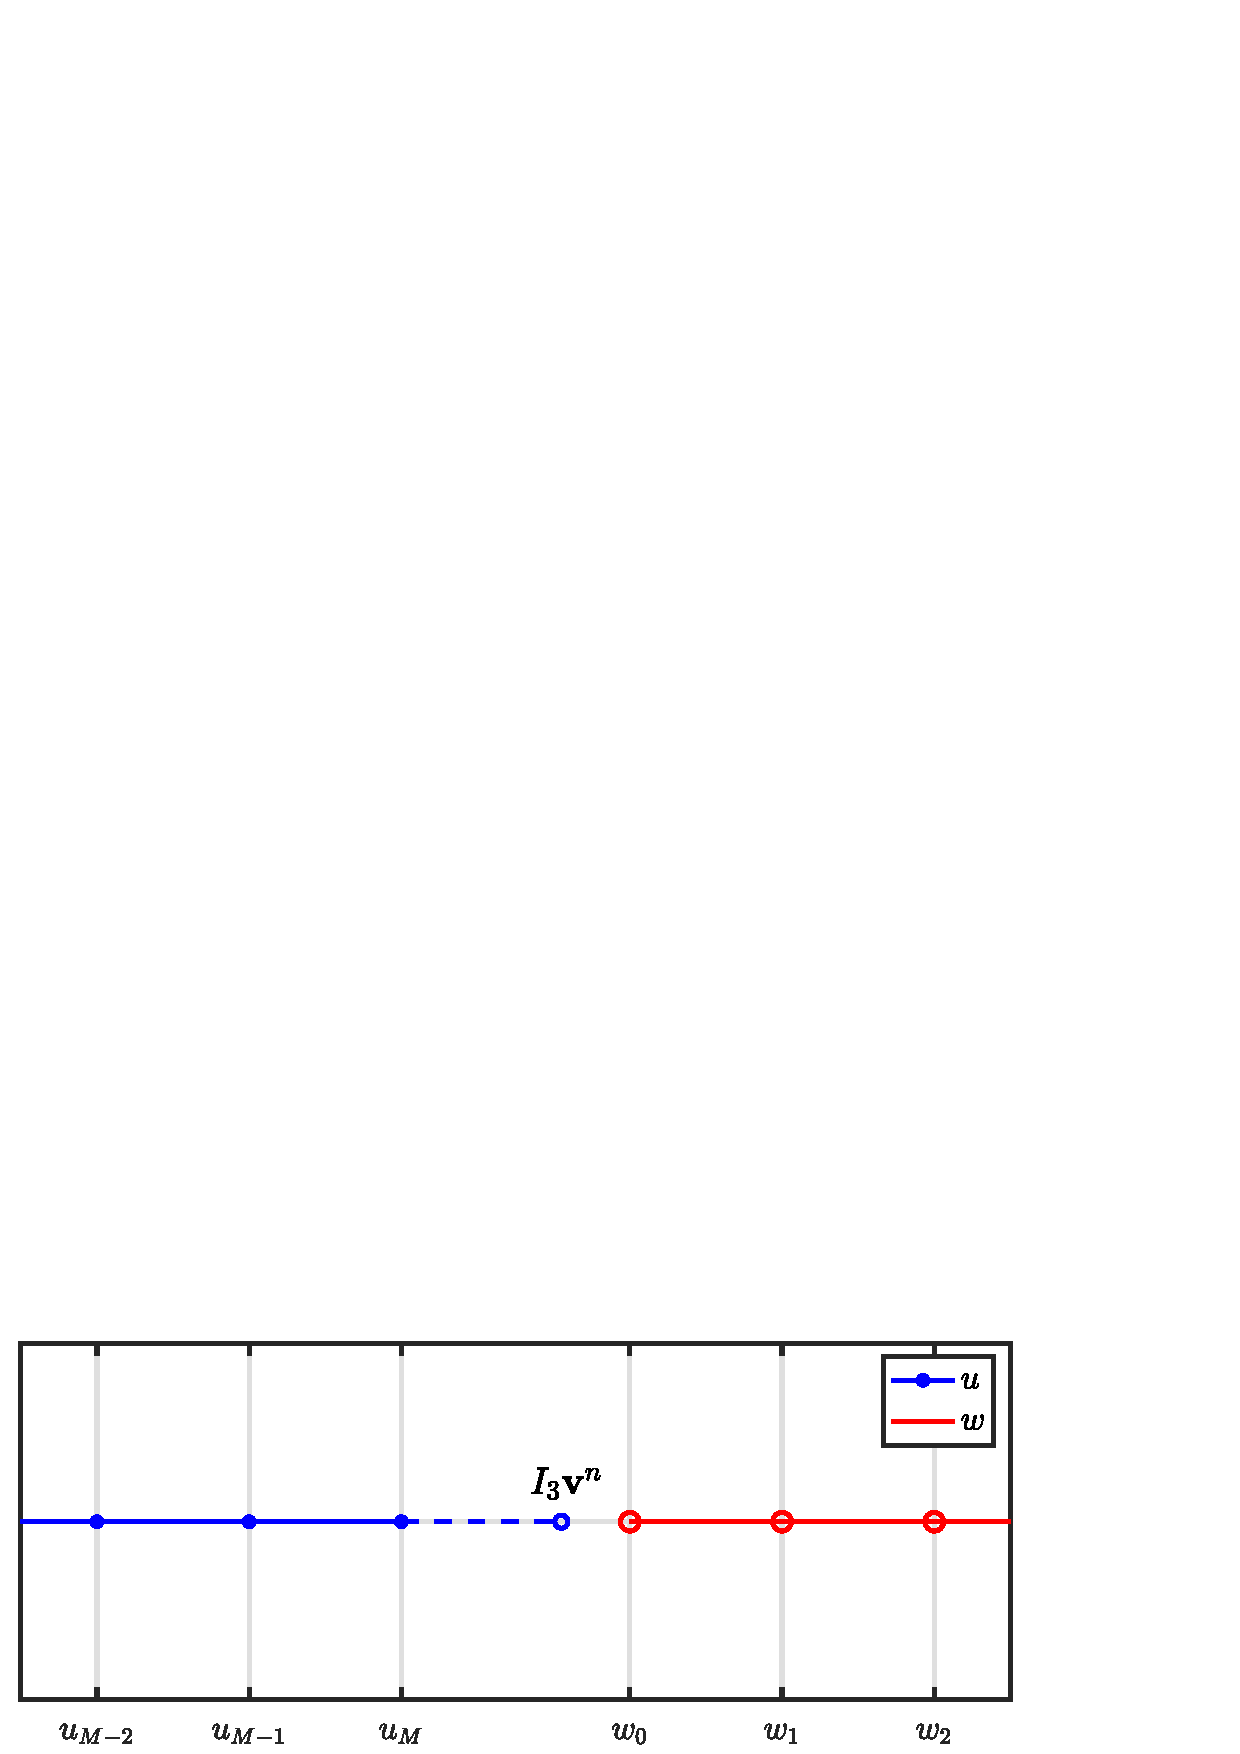
\includegraphics[width=0.8\columnwidth]{addingGridPoint4}
\caption{\label{fig:addingPoint}{The moment when a point is added to $\mathbf{u}$ at location $x_{u_M} + h$ in Eq. \eqref{eq:addingPoint}. This figure shows an extreme case where this location is far from $x_{w_0}$, i.e., $\alpha' \not\approx 0$ in Eq. \eqref{eq:customIp}.}}
\end{figure} 

Except in the case of extremely quick parameter variations, $\alpha'$ in Eq. \eqref{eq:customIp} is expected to be close to zero, i.e., $x_{u_M}^n + h \approx x_{w_0}^n$, meaning that $I_3 \approx [0, 0, 1, 0]$. This makes sense by looking at Figure \ref{fig:twoFreeStringsGridZoomed}, as exactly when the boundary points $u_M^n$ and $w_0^n$ surpass the virtual points $w_{-1}^n$ and $u_{M+1}^n$, these are going to be close to overlapping.

Removing grid points happens when $c$, and consequently $h$, is increased and $x_{u_M}^n \geq x_{w_0}^n$ (or $\lfloor N^n\rfloor < \lfloor N^{n-1}\rfloor$). Compared to adding grid points, removing these is slightly more straightforward as points are simply removed from $\mathbf{u}$ and $\mathbf{w}$ (again for both $n$ and $n-1$) in an alternating fashion
\begin{equation}\label{eq:removingPoint}
\begin{cases}
    \mathbf{u}^n = [u_0^n, u_1^n ..., u_{M-1}^n]^T & \text{if $N^n$ is even}, \\
     \mathbf{w}^n = [w_1^n, w_2^n ..., w_{M_w}^n]^T & \text{if $N^n$ is odd}.
    \end{cases}
\end{equation}

A problem that arises from simply removing a grid points, is that it is possible that $u_M^n \not\approx w_0^n$ at the time of removal. As $x_{u_M}^n \approx x_{w_0}^n$ at the time of removal (except for extremely quick parameter variations), this violates the rigid connection in \eqref{eq:rigid} and causes audible artefacts. A method of displacement correction is proposed that decreases the relative displacement of the inner boundaries the closer their grid-locations are together, i.e., the closer $\alpha$ in \eqref{eq:alphaDef} is to 0:
\begin{equation}\label{eq:dispCorr}
    \begin{aligned}
    u_M^n := u_M^n +\beta (w_0^n - u_M^n),\\
    w_0^n := w_0^n - \beta  (w_0^n - u_M^n),
    \end{aligned}
\end{equation}
with
\begin{equation}\label{eq:betaDef}
    \beta(\epsilon) = \frac{(1-\alpha)^\epsilon}{2}
\end{equation}
where $\epsilon \geq 1$ is a tunable parameter. A lower $\epsilon$ decreases the chance of artifacts but will have a greater low-passing effect on the system. For low-speed changes, using $\sim 1000$ samples for removing one grid point, $\epsilon \approx 30$ ensures that $u_M^n \approx w_0^n$ and already suffices to remove artefacts arising from point removal.

Until now, only adding and removing points in the center of the system has been considered. This location could be moved anywhere along the grid, the limit being one point from the boundary. Furthermore, one does not have to add and remove points from $\mathbf{u}$ and $\mathbf{w}$ in an alternating fashion as in \eqref{eq:addingPoint}, but can just add and remove from (fx.) $\mathbf{u}$ leaving $\mathbf{w}$ the same size throughout the simulation. In the extreme case where $M = \lfloor N\rfloor - 1$ and $M_w = 1$ (leaving $\mathbf{w}$ with only one moving grid point, $w_0^n$) the method still works.
% 
% \SWcomment[The following applies to odd-ordered Lagrange interpolators $\rightarrow$] The location at where points are added and removed greatly influences the behaviour of the system, especially in the higher frequencies (see Section \ref{sec:results}). The best behaviour is obtained when the location is as close to a boundary as possible. 

\subsection{Summary}
Here, Section \ref{sec:proposedMethod} is summarised and describes the final version of the proposed method.

The complete system consists of two grid functions $u_l^n$ and $w_l^n$ of size of size $M$ and $M_w$. Knowing that $\lambda=1\ \forall n$, Eq. \eqref{eq:updateEq}, written for both grid functions, becomes 
\begin{subequations}\label{eq:uwUpdates}
    \begin{align}
        u_l^{n+1} &= u_{l+1}^n + u_{l-1}^n - u_l^{n-1},\label{eq:uUpdate}\\
        w_l^{n+1} &= w_{l+1}^n + w_{l-1}^n - w_l^{n-1}\label{eq:wUpdate},
    \end{align}
\end{subequations}
%
Due to the Dirichlet boundary condition in \eqref{eq:discreteDirichlet} imposed on the outer boundaries of the system, $u_0^n$ and $w_{M_w}^n$ are $0$ at all times and are not included in the calculation. The range of calculation for Eq. \eqref{eq:uUpdate} and \eqref{eq:wUpdate} then become $l = [1, \hdots, M]$ and $l = [0, \hdots, M_w - 1]$ respectively. 

The inner boundaries are calculated using
\begin{subequations}
    \begin{align}
        u_M^{n+1} &= u_{M+1}^n + u_{M-1}^n - u_M^{n-1},\\
        w_0^{n+1} &= w_{-1}^n + w_{2}^n - w_0^{n-1}.
    \end{align}
\end{subequations}
%
where virtual grid points $u_{M+1}^n$ and $w_{-1}^n$ can be calculated using Eq. \eqref{eq:connectionInterpol}.

Then, when $\lfloor N^n \rfloor > \lfloor N^{n-1} \rfloor$ a point is added to $\mathbf{u}^n$ and $\mathbf{u}^{n-1}$ (or $\mathbf{w}^n$ and $\mathbf{w}^{n-1}$) using Eq. \eqref{eq:addingPoint}, and when $\lfloor N^n \rfloor <\lfloor N^{n-1} \rfloor$ a point is removed from the same vectors using Eq. \eqref{eq:removingPoint}. In order to prevent audible artefacts when increasing $c$ (and thus decreasing $N$), the displacement correction in \eqref{eq:dispCorr} is proposed to ensure that the inner boundaries have a similar displacement when one of them is removed.

Finally, using $\mathbfcal{U}$ from Eq. \eqref{eq:fullState} the total system can then be compactly written in matrix form as
\begin{equation}\label{eq:totalSystem}
    \mathbfcal{U}^{n+1} = 
    \mathbf{B} 
    \mathbfcal{U}^n
    - \mathbfcal{U}^{n-1}
\end{equation}
with $\lfloor N\rfloor \times \lfloor N\rfloor$ matrix
\begin{equation}\label{eq:bMat}\small
    \mathbf{B} = \begin{bmatrix}[cccc|cccc]
        & \ddots  &\ddots & & & & 0 & \\
          & 1 & 0 & 1 & & & & \\
         & & 1 & \frac{\alpha - 1}{\alpha + 1} - \beta  & 1 + \beta & -\frac{\alpha - 1}{\alpha + 1} & \\ \cline{2-7}
         & & -\frac{\alpha - 1}{\alpha + 1} & 1 + \beta & \frac{\alpha - 1}{\alpha + 1} - \beta  & 1 & & \\
            & & & &1 & 0 & 1  \\
            & 0 & &  &  &\ddots & \ddots &
       \end{bmatrix}
\end{equation}
%
% \begin{equation}\small
%     \mathbf{B} = \begin{bmatrix}[ccccccc|cc]
%     & &\ddots &\ddots & \ddots  & & \mathbf{0} & & \\
%      & & &1 & 0 & 1 & & \mathbf{0} & \\
%      & & &  & 1 & 0 & 1 & & \\
%      & &\mathbf{0} &  & \mathbfcal{A}_{1, 2}\alpha_\text{I} &\mathbfcal{A}_{1, 2}\beta_\text{I} + 1 &\mathbfcal{A}_{1, 2}\gamma_\text{I} & \mathbfcal{A}_{1, 1}(\gamma_\text{I}-\alpha_\text{I})& \\ \cline{2-8}
%      & & \mathbf{0} & &\mathbfcal{A}_{2, 2}\alpha_\text{I} &\mathbfcal{A}_{2, 2}\beta_\text{I}&\mathbfcal{A}_{2, 2}\gamma_\text{I} & \mathbfcal{A}_{2,1}(\gamma_\text{I} - \alpha_\text{I}) & 
%     \end{bmatrix}
% \end{equation}
%
Notice that when $\alpha$ approaches $1$, $\mathbf{B}$ will reduce to a matrix with ones on the diagonals next to the main diagonal and zeros elsewhere, which translates directly to the usual situation in Eq. \eqref{eq:updateEq} with $N = M + M_w + 1$. 

\subsection{Implementation}
When implementing this method, it is important not to change the grid as the scheme is calculated. I.e., the same $\alpha$ and $\beta$ need to be used to calculate $u^n_l$ and $w^n_l$ at time index $n$ for all $l$.

% \begin{algorithmic}[ht]
% \vspace{1em}
% \fbox{\parbox{0.8\linewidth}{
% \setstretch{1.5}
% \While{application is running}
% \State Wavespeed $c$ is changed
% \If{$\lfloor N^n\rfloor > \lfloor N^{n-1} \rfloor$}
%   \State Add point (Eq. \eqref{eq:addingPoint})
% \ElsIf{$\lfloor N^n\rfloor < \lfloor N^{n-1} \rfloor$}
%   \State Remove point (Eq. \eqref{eq:removingPoint})
% \EndIf
%     \State Calc. $\alpha$ and $\beta$ (Eqs. \eqref{eq:alphaDef} and \eqref{eq:betaDef})
%     \State Calc. scheme (Eq. \eqref{eq:totalSystem})
%     \State Retrieve output
%     \State Update FDS States
% \EndWhile}}
% % \caption{Pseudo code showing the order of calculation \label{alg:calcOrder}}
% \end{algorithmic}

\SWcomment[going to include some pseudocode here to rather than the list below]
\begin{itemize}
    \item Wavespeed is changed
    \item Check whether $\lfloor N^n\rfloor \neq \lfloor N^{n-1} \rfloor$
    \begin{itemize}
        \item If so add/remove point using \eqref{eq:addingPoint} or \eqref{eq:removingPoint}
    \end{itemize}
    \item Calculate $\alpha$ and $\beta$ in \eqref{eq:bMat} using \eqref{eq:alphaDef} and \eqref{eq:betaDef}.
    \item Calculate scheme \eqref{eq:totalSystem}
    \item Retrieve output
    \item Update states
\end{itemize}

\parskip 18pt
\section{Analysis and Results}\label{sec:results}
% \subsection{Expected behaviour}
This section shows the analysis of the system presented in the previous section and its behaviour.

% \subsection{Static}
\subsection{Frequency}
In order to determine whether the proposed method yields an output with the correct frequency content in the static case, a spectrum is taken of the system's output. The system with $N=15.5$ (so $\alpha = 0.5$ in \eqref{eq:bMat}) at a sample rate of $f_\text{s} = 44100$ Hz is compared to the same system with $f_\text{s} = 88200$ Hz resulting in $N=31$ ($\alpha = 0$) for the same $f_0$ according to Eq. \eqref{eq:fundamentalFreq}. See Figure \ref{fig:spectra}.

\begin{figure}[ht]
    \centering
%% \reprintcolumnwidth is the same in preprint and reprint for
%% ease of use for authors:
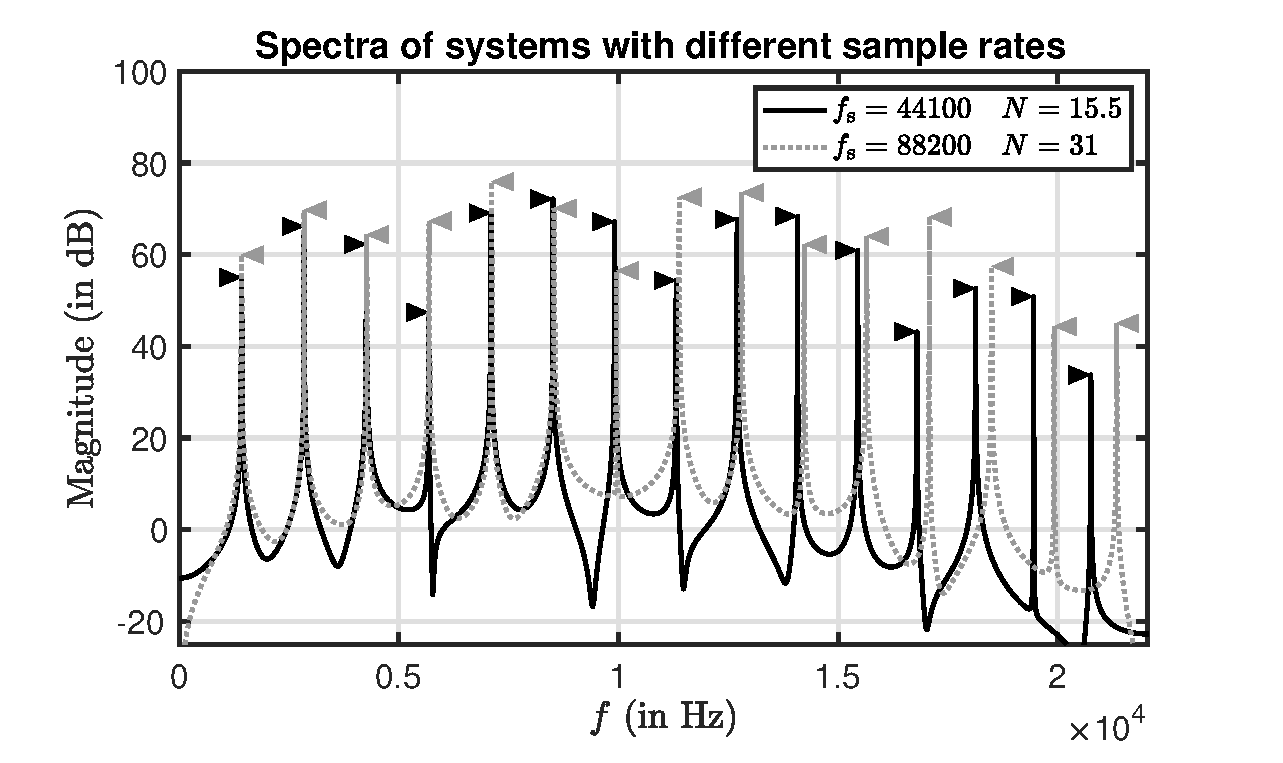
\includegraphics[width=0.8\columnwidth]{spectraDoubleSampleRateQuadratic}
\caption{\label{fig:spectra}{A system with $N = 15.5$ at $f_\text{s} = 44100$} compared to a system with $N = 31$ at $f_\text{s} = 88200$. Both are supposed to have the same fundamental frequency $f_0$ according to Eq. \eqref{eq:fundamentalFreq}.}
\end{figure} 

As expected, the output of the system at integer $N = 31$ contains partials at perfect integer multiples of $f_0$ (Eq. \eqref{eq:fundamentalFreq}). When this is compared to the output of the system with $N = 15.5$, one can observe that the lower partials are nearly perfectly overlapping, whereas higher partials exhibit slight downwards deviations, exponentially increasing with frequency.

% \subsection{Dynamic}
For a more detailed look at the behaviour of the system when $c$ is changed dynamically, a modal analysis can be performed on system \eqref{eq:totalSystem}. For slow variations of $c$, the modal frequency of the $p$'th mode can be retrieved as
\begin{equation}\label{eq:modalAnalysis}
    f_p \approx \frac{1}{2\pi k}\cos^{-1}\left(\frac{1}{2}\text{eig}_p(\mathbf{B})\right).
\end{equation}

As a test case, the wave speed is dynamically varied from $c = 2940$ ($N = 15$) to $c = 2205$ ($N = 20$), changing $\mathbf{B}$ and thus the modal frequencies over time. The displacement correction presented in Eq. \eqref{eq:dispCorr} is not included in this analysis ($\epsilon \gg 1$), but will be elaborated on in Section \ref{sec:dispCorrRes}. The results of the analysis are shown in Figure \ref{fig:modalAnalysis}. Figure \ref{fig:spectrogram} shows the resulting spectrogram of the system excited at $n=0$ with a narrow raised cosine and the output retrieved at $u_1$.

\begin{figure}[ht]
    \centering
%% \reprintcolumnwidth is the same in preprint and reprint for
%% ease of use for authors:
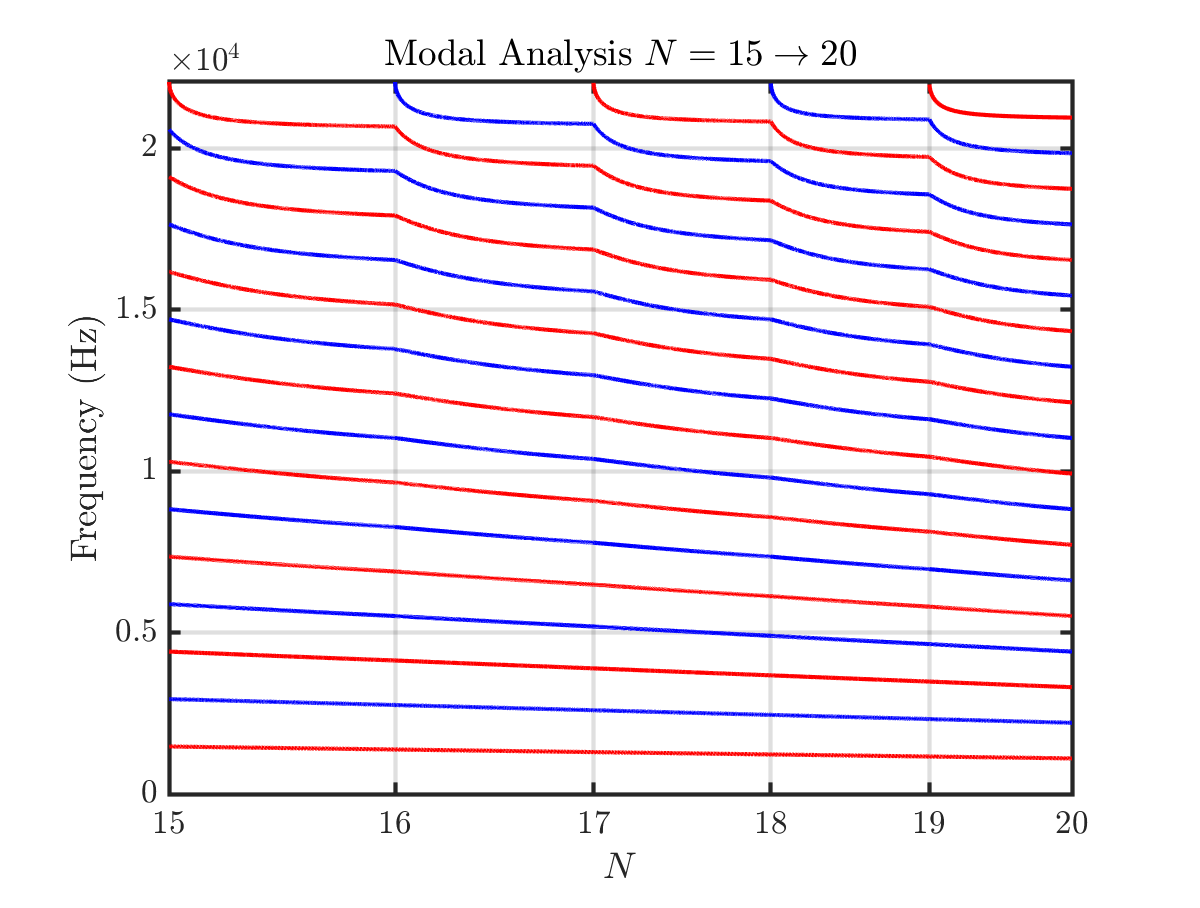
\includegraphics[width=0.8\columnwidth]{modalAnalysisQuadratic}
\caption{\label{fig:modalAnalysis}{Modal analysis of system \eqref{eq:totalSystem} using \eqref{eq:modalAnalysis}. The wave speed is reduced from $c = 2940$ ($N = 15$) to $c = 2205$ ($N = 20$).}}
\end{figure} 
\begin{figure}[ht]
    \centering
%% \reprintcolumnwidth is the same in preprint and reprint for
%% ease of use for authors:
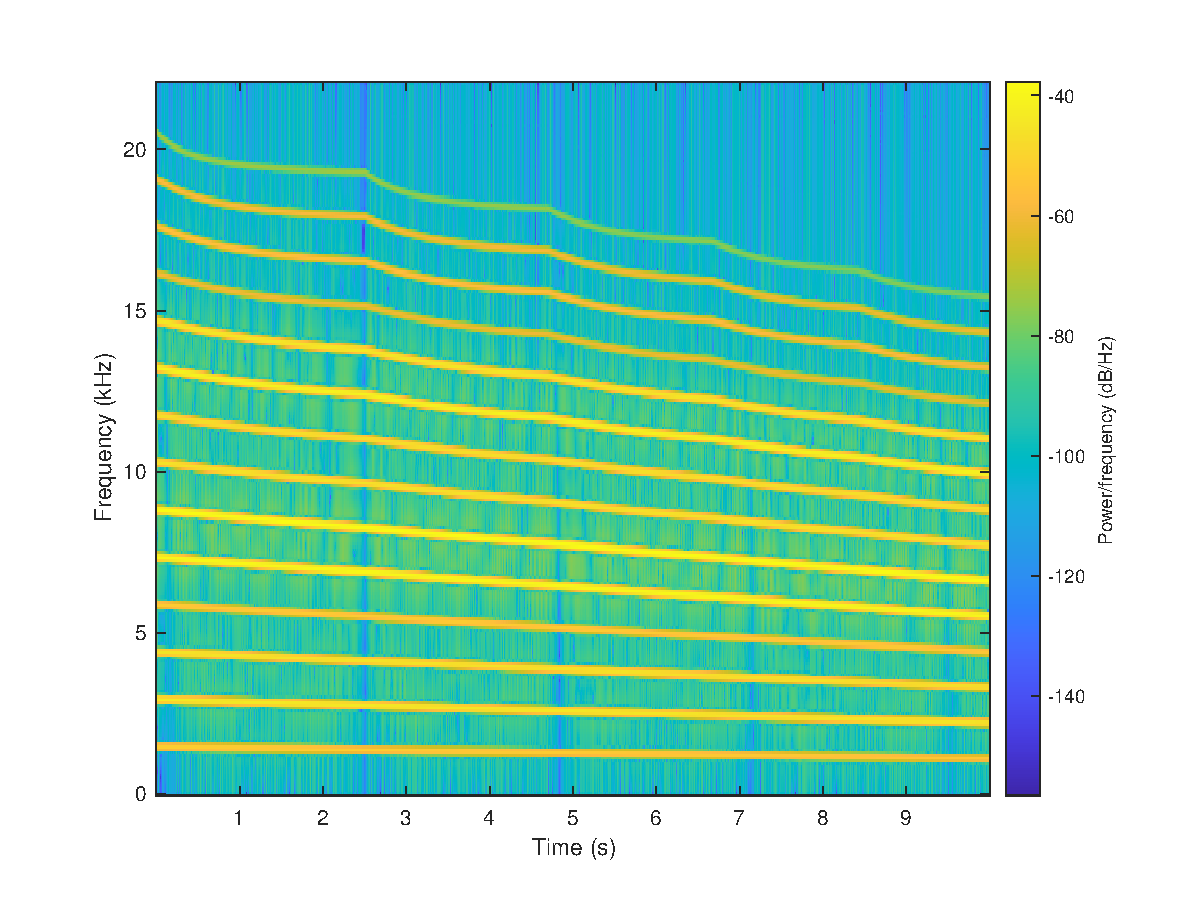
\includegraphics[width=0.8\columnwidth]{specQuadratic}
\caption{\label{fig:spectrogram}{System output. The sound output follows the same pattern as predicted by the analysis shown in Figure \ref{fig:modalAnalysis}.}}
\end{figure} 

In the following \SWcomment[came up with this measure myself.. it made sense to me for measuring harmonic deviation / inharmonicity. Please let me know if you know a better measure or something I can reference]
\begin{equation}
    \varepsilon_p = \frac{f_p - pf_0}{f_0}\quad \text{[\%]}
\end{equation}
is used to calculate the harmonic deviation of mode $p$ from an integer multiple of the fundamental. Furthermore, the lowest mode generated by the analysis is referred to as $f_1$ and should ideally be equal to $f_0$ calculated using Eq. \eqref{eq:fundamentalFreqCont}.

The first thing one can observe from Figure \ref{fig:modalAnalysis} is that the frequencies of the modes decrease as $c$ decreases. The lower the mode, the more linear this decrease happens. Between $N = 15$ and $N = 16$, $f_1$ maximally deviates by $-0.12$ Hz or $\varepsilon_1 = -0.008\%$. In this same interval $f_{15}$ maximally deviates by $-827.15$ Hz or $\varepsilon_{15} = -57\%$. This deviation for mode number $p$ gets progressively less as $N$ increases. The maximum deviation for the highest mode number $f_{\lfloor N\rfloor}$, however, gets larger with a larger $N$, with $\text{max}(\varepsilon_{\lfloor N \rfloor})$ approaching $-100\%$ for extremely large values of $N$ ($>1000$). These deviations only happen between integer values of $N$ where at integer $N$ all modes are perfect integer multiples of $f_0$ and $\varepsilon_p = 0 \%$ for all $p$.

Experiments with higher even-ordered Lagrange interpolators shows that $\varepsilon_p$ becomes smaller, but not by a substantial amount. The quadratic interpolator has thus been chosen for being simpler and more flexible while not being substantially worse than higher order interpolators.

Another observation from Figure \ref{fig:modalAnalysis} is that there are always $\lfloor N \rfloor$ modes present, corresponding to the number of moving points of the system. As can be seen from the spectrum in Figure \ref{fig:spectrogram} the highest mode is not excited. When an implementation of the system using this method, with wave speed $c = 2940$ m/s (static) is compared to a normal implementation of the 1D wave equation (shown in Section \ref{sec:FDTD}) with the same wavespeed, identical outputs are observed, even though the latter has $N-1$ moving points. This proves that at integer $N$ the method reduces to the normal case. If the system is excited when $N$ is not an integer, the highest mode will also be excited.

Using the quadratic interpolation from \eqref{eq:connectionInterpol}, or any other even-ordered Lagrange interpolator for that matter, the modal behaviour of the system does not change based on location. Experiments done with odd-ordered Lagrange interpolators showed that better behaviour is observed when points are added / removed closer to the boundaries. 

\subsection{Displacement Correction}\label{sec:dispCorrRes}
(FIR) Comb filtering effect where resonances appear depending on the location of correction. Middle has least

\subsection{Limit on Speed of Change}
The method presented in this paper can only add or remove a maximum one point per sample using Eqs. \eqref{eq:addingPoint} and \eqref{eq:removingPoint}. The speed of decreasing $f_0$ according to \eqref{eq:fundamentalFreq} is thus limited by the following condition
\begin{equation}\label{eq:pointCondition}
    |N^n - N^{n-1}| \leq 1. 
\end{equation}
Though this is the maximal limitation on speed, a much lower limitation needs to be placed 
% Notes:
% In the case that $\alpha = 0$ in Eq. \eqref{eq:totalSystem} (and thus $x_{u_M} = x_{w_0}$), one could go up to adding two points at a time by adding $u_{M+1}^n$ according to Eq. \eqref{eq:addingPoint} and adding an extra point $u_{M+2}^n$ using \eqref{eq:calcVirtualGridPoints} (in this case $u_{M+2}^n = w_0^n$). This would, however, not work if $\alpha \neq 0$, as a point added to $\mathbf{u}^n$ with $x_\text{i} < w_0$ needs interpolator \eqref{eq:customIp} and $\alpha'$ would be greater than $1$. As Eq. \eqref{eq:customIp} only works if $0\leq \alpha' \leq 1$, it is best to abide condition \eqref{eq:pointCondition} to be safe. 

% No speed limit if
% \begin{equation}
%     \text{floor}(N^n) = \text{floor}(N^{n-1})\Rightarrow M^n = M^{n-1},
% \end{equation}
% i.e., if no points are added or removed from the system. 
\parskip 18pt
\section{Discussion}
To decide whether the proposed method works satisfactory, the results presented in the previous section are compared to the method requirements listed in Section \eqref{sec:methodReq}. 

The fact that he highest mode is not excited is probably due to the restriction imposed on the two moving but connected points through the rigid connection.


All issues with the proposed method happen in higher frequencies. Physical processes usually lose the highest frequencies first

Due to high-frequency losses in physical systems. 

Higher modes

As can be seen from the figure, the lower harmonic partials of both systems line up almost exactly before the partials interpolated start to deviate towards the lower end of the spectrum.

($<0.2\%$ of their respective frequency, $<1.3\%$ of the fundamental $f_0$). 


Applications could be non-linear systems where parameters are modulated based on the state of the system. 

The proposed method does not provide the exact solution to the problem, but does circumvent the need for upsampling and higher orders of computations necessary to approximate this solution. Even though interpolation needs to happen, the drawbacks of full-grid interpolation can be avoided by not `listening' to the location where points are added but rather closer to the boundary. If one wants to listen to the center, the location where points are added or removed can easily be changed.


frequency domain, the locations of the partials comparing the discrete 1D wave with $N = 30.5$ and $f_\text{s} = 44100$ (interpolation needs to happen) with $N = 61$ and $f$ 

If the amount that a parameter changes within a small enough period of time (give values here, hopefully referring back to the results) the fact that points are added at a specific location (rather than distributed over the grid) will not matter as... 

The 


\parskip 18pt
\section{Conclusion and Future Work}

Future work includes creating an adaptive version of the displacement correction that changes its effect depending on the speed at which the grid is changed.  
Though this method has only been presented using the 1D wave equation it could potentially be applied to any kind of 1D FDS 


%References
\bibliographystyle{cmj}
\bibliography{cmjbib}

\end{document}
